% =========================================================
% Rapport PFE/Stage - IIT (Template ENET'COM)
% Projet CRM Full-Stack + Mobile + IA Chatbot
% =========================================================

\documentclass[12pt,oneside,a4paper]{Enetcom-PFE-Report-dissertation}
\graphicspath{{images/}}

%%%%%%%%%%%%%%%%%%%%%%%%%%%%%%%%%%%%%%%%%%%%%%%%%%%%%%%%%%%
% Package pour \checkmark
\usepackage{amssymb}
\usepackage{longtable}
\usepackage{booktabs}
\usepackage{float}
\usepackage{listings}
\usepackage{pifont}

%%%%%%%%%%%%%%%%%%%%%%%%%%%%%%%%%%%%%%%%%%%%%%%%%%%%%%%
% TikZ — UML Use Case Diagram styles
%%%%%%%%%%%%%%%%%%%%%%%%%%%%%%%%%%%%%%%%%%%%%%%%%%%%%%%
\usetikzlibrary{positioning, arrows.meta, shapes.geometric, fit, calc, backgrounds}

% Use case ellipse
\tikzset{
  usecase/.style={
    draw, ellipse, align=center, font=\small,
    inner xsep=4pt, inner ysep=2pt,
    minimum width=2.6cm, minimum height=1cm,
    text width=2.4cm
  },
  usecaseSmall/.style={
    draw, ellipse, align=center, font=\footnotesize,
    inner xsep=3pt, inner ysep=2pt,
    minimum width=2.2cm, minimum height=0.85cm,
    text width=2cm
  },
  % System boundary
  systemboundary/.style={
    draw, rectangle, rounded corners=3pt,
    inner sep=12pt, thick, fill=blue!3
  },
  % Include / Extend arrows
  include/.style={
    ->, dashed, >=Stealth,
    shorten >=2pt, shorten <=2pt
  },
  extend/.style={
    ->, dashed, >=Stealth,
    shorten >=2pt, shorten <=2pt
  },
  % Association line
  assoc/.style={
    -, shorten >=2pt, shorten <=2pt
  },
}

% Stick figure command: \umlactor{node name}{x,y}{label}
\newcommand{\umlactor}[3]{%
  \begin{scope}[shift={(#2)}]
    \draw[thick] (0,0.6) circle (0.18);          % head
    \draw[thick] (0,0.42) -- (0,0);              % body
    \draw[thick] (-0.25,0.32) -- (0,0.18) -- (0.25,0.32);  % arms
    \draw[thick] (-0.2,-0.3) -- (0,0) -- (0.2,-0.3);       % legs
    \node[below, font=\small\bfseries] at (0,-0.35) {#3};
    \coordinate (#1) at (0,0.18);
  \end{scope}
}

% Config listings
\lstset{
    basicstyle=\ttfamily\small,
    keywordstyle=\color{blue}\bfseries,
    stringstyle=\color{green!50!black},
    commentstyle=\color{gray}\itshape,
    breaklines=true,
    frame=single,
    backgroundcolor=\color{gray!5},
    numbers=left,
    numberstyle=\tiny\color{gray},
    tabsize=2,
    showstringspaces=false,
}

%%%%%%%%%%%%%%%%%%%%%%%%%%%%%%%%%%%%%%%%%%%%%%%%%%%%%%%
% MÉTADONNÉES DU RAPPORT
%%%%%%%%%%%%%%%%%%%%%%%%%%%%%%%%%%%%%%%%%%%%%%%%%%%%%%%

\newcommand{\reportAuthor}{%
  Mahdi \textsc{CHAKROUN}%
}

\newcommand{\reportTitle}{%
   Conception et Développement d'un Système CRM Full-Stack \\ 
   avec Portail Client, Application Mobile et Chatbot IA%
}

\newcommand{\reportSubject}{%
   Rapport de Stage de Fin d'Études%
}

\newcommand{\dateSoutenance}{%
  2026%
}

\newcommand{\studyDepartment}{%
  Génie Logiciel et Informatique Décisionnelle%
}

\newcommand{\ENETCOM}{%
  Institut Polytechnique Privé des Sciences Avancées de Sfax%
}

\newcommand{\codePFE}{%
}

%%%%%%%%%%%%%%%%%%%%%%%%%%%%%%%%%%%%%%%%%%%%%%%%%%%%%%%
% JURY
%%%%%%%%%%%%%%%%%%%%%%%%%%%%%%%%%%%%%%%%%%%%%%%%%%%%%%%

\newcommand{\juryPresident}{%
  Mr [Nom] \textsc{[Prénom]}%
}
\newcommand{\juryPresidentDesc}{%
  Président%
}

\newcommand{\juryMemberOne}{%
  Mr Ahmed \textsc{KHARAT}%
}
\newcommand{\juryMemberOneDesc}{%
  Encadrant académique%
}

\newcommand{\juryMemberTwo}{%
  Mr [Nom] \textsc{[Prénom]}%
}
\newcommand{\juryMemberTwoDesc}{%
  Rapporteur%
}

%%%%%%%%%%%%%%%%%%%%%%%%%%%%%%%%%%%%%%%%%%%%%%%%%%%%%%%
% COMMANDES UTILITAIRES
%%%%%%%%%%%%%%%%%%%%%%%%%%%%%%%%%%%%%%%%%%%%%%%%%%%%%%%

\newcommand{\specialcell}[1]{%
  \begin{tabularx}{\textwidth}{@{}X@{}}#1\end{tabularx}%
}

\newcommand{\PlaceholderFigure}[5]{%
  \begin{figure}[H]
    \centering
    \fbox{%
      \begin{minipage}[c][#2][c]{#1}
        \centering
        \textbf{#3}\par
        \vspace{0.3cm}
        \small #4
      \end{minipage}
    }
    \caption{#3}
    \label{#5}
  \end{figure}
}

\newcommand{\MyCommand}{%
  Does nothing really%
}


%%%%%%%%%%%%%%%%%%%%%%%%%%%%%%%%%%%%%%%%%%%%%%%%%%%%%%%%%%%
% CAPTIONS TABLEAUX EN HAUT
%%%%%%%%%%%%%%%%%%%%%%%%%%%%%%%%%%%%%%%%%%%%%%%%%%%%%%%%%%%
\usepackage{caption}
\captionsetup[table]{position=above}

%%%%%%%%%%%%%%%%%%%%%%%%%%%%%%%%%%%%%%%%%%%%%%%%%%%%%%%%%%%
% JUSTIFICATION PARFAITE
%%%%%%%%%%%%%%%%%%%%%%%%%%%%%%%%%%%%%%%%%%%%%%%%%%%%%%%%%%%
\usepackage{microtype}
\microtypesetup{protrusion=true,expansion=true}

\usepackage{ragged2e}
\AtBeginDocument{\justifying}

\tolerance=1000
\emergencystretch=1em
\hyphenpenalty=50
\exhyphenpenalty=50

%%%%%%%%%%%%%%%%%%%%%%%%%%%%%%%%%%%%%%%%%%%%%%%%%%%%%%%%%%%
% Fix langue FR
%%%%%%%%%%%%%%%%%%%%%%%%%%%%%%%%%%%%%%%%%%%%%%%%%%%%%%%%%%%
\addto\captionsfrench{%
  \renewcommand{\chaptername}{Chapitre}%
  \renewcommand{\contentsname}{TABLE DES MATIÈRES}%
  \renewcommand{\listfigurename}{LISTE DES FIGURES}%
  \renewcommand{\listtablename}{LISTE DES TABLEAUX}%
  \renewcommand{\figurename}{Figure}%
  \renewcommand{\tablename}{Tableau}%
}

\providecommand{\mtcname}{}
\providecommand{\mtcSname}{}
\renewcommand{\mtcname}{Sommaire}
\renewcommand{\mtcSname}{Sommaire}
\mtcselectlanguage{french}

%%%%%%%%%%%%%%%%%%%%%%%%%%%%%%%%%%%%%%%%%%%%%%%%%%%%%%%%%%%
% PDF metadata
%%%%%%%%%%%%%%%%%%%%%%%%%%%%%%%%%%%%%%%%%%%%%%%%%%%%%%%%%%%
\hypersetup{%
  pdftitle={\reportTitle~-~\reportSubject},%
  pdfauthor={\reportAuthor},%
  pdfsubject={\reportSubject},%
  pdfkeywords={CRM}{React}{FastAPI}{Docker}{Mobile}{IA}{RAG}%
}

\dominitoc

\begin{document}

\makeatletter
\let\oldraggedright\raggedright
\renewcommand{\raggedright}{\justifying}
\let\RaggedRight\justifying
\makeatother
\justifying

\setstretch{1.2}
\setlength{\parskip}{0pt}
\setlength{\parindent}{1.2em}

% ------------------------------------------------------------
% Couverture
% ------------------------------------------------------------
\thispagestyle{empty}
\begin{titlepage}
\begin{center}

{%
  \fontsize{9pt}{9pt}\selectfont%
  \begin{tabularx}{\textwidth}{ @{} p{0.35\textwidth} @{} p{0.02\textwidth} @{} p{0.3\textwidth} @{} p{0.02\textwidth} @{} p{0.35\textwidth} @{} }
    \centering%
    Republique Tunisienne\\%
    Ministère de l'Enseignement Supérieur \\%
    et de la Recherche Scientifique\\%
    \begin{spacing}{1}
    \end{spacing}
    \begin{spacing}{0.05}
    \noindent
    \rule{50pt}{0.75pt}\\
    \rule{50pt}{0.75pt}
    \end{spacing}
    \begin{spacing}{1.4}
    \end{spacing}
    Université de Sfax\\%
    \begin{spacing}{1}
    \end{spacing}
    \begin{spacing}{0.05}
    \noindent
    \rule{50pt}{0.75pt}\\
    \rule{50pt}{0.75pt}
    \end{spacing}

    & &
    \centering%
    \multirow{2}{\linewidth}{%
      \centering%
      
\includegraphics[width=4.94cm, height=2.56cm]{images/poly_logo.png}%
    }%
    & &
    \vspace{10pt}
    \centering%
    \textbf{%
    \\%
    Licence en :\\%
    }
    Informatique de Gestion\\%
    \tabularnewline%
    \centering%
    \begin{spacing}{0.3}
    \end{spacing}
    Institut Polytechnique Privé des\\%
    Sciences Avancées de Sfax%
    & & & &
    \tabularnewline%
    \arrayrulecolor{reportType}%
    \specialrule{0.75pt}{2pt}{0pt}%
    \specialrule{2.00pt}{1pt}{0pt}%
  \end{tabularx}
}

\vspace{14pt}
{%
  \renewcommand*{\familydefault}{\defaultFont}
  \fontsize{34pt}{34pt}\selectfont%
  Rapport de Stage de\\%
  Fin d'Études\\%
}

\vspace{18pt}
\renewcommand*{\familydefault}{\defaultFont}
\fontsize{13.5pt}{13.5pt}\selectfont%
\textbf{\textit{Réalisé au sein de :}} \textbf{FRS}\\

% Logo FRS
\vspace{18pt}

\includegraphics[width=8.2cm]{images/FRS_logo.jpg}\\

\vspace{16pt}
{%
  \begin{spacing}{0.05}
    \rule{260pt}{2pt}\\
    \rule{260pt}{0.75pt}\\
  \end{spacing}
  \renewcommand*{\familydefault}{\defaultFont}
  \fontsize{15.5pt}{15.5pt}\selectfont%
  \vspace{12pt}
  \textbf{Titre du projet :}\\[6pt]
  \textbf{
  Conception et Développement d'un Système CRM Full-Stack\\
  avec Portail Client, Application Mobile et Chatbot IA\\
  }
  \vspace{10pt}
  \begin{spacing}{0.05}
    \rule{260pt}{0.75pt}\\
    \rule{260pt}{2pt}\\
  \end{spacing}
}

\vspace{18pt}
\textbf{\textit{Préparé par}}\\
\vspace{8pt}
{%
  \fontsize{17pt}{17pt}\selectfont%
  \textbf{Mahdi CHAKROUN}\\
}%

\vspace{18pt}
\begin{tabularx}{\textwidth}{@{} >{\centering\arraybackslash}X >{\centering\arraybackslash}X @{}}
\textbf{Encadrant académique :} & \textbf{Encadrant professionnel :} \\
\textbf{Ahmed KHARAT} & \textbf{Ghassen BAKLOUTI} \\
\end{tabularx}

\vspace{16pt}
Année Universitaire : 2025 / 2026\\

\vfill
\end{center}
\end{titlepage}


\pagenumbering{roman}

\chapter*{DÉDICACE}
\thispagestyle{MyStyle}

\begin{center}
{\huge A}vec l'expression de ma reconnaissance, je dédie ce modeste travail à ceux qui, quels que soient les termes embrassés, je n'arriverai jamais à leur exprimer mon amour sincère.\\[1.5em]

{\huge A} l'homme, mon précieux don de Dieu, à qui je dois ma vie,\\ ma réussite et tout mon respect : \textbf{mon cher père}.\\[1em]

{\huge A} la femme qui a souffert sans me laisser souffrir, qui n'a jamais dit non à mes exigences et qui n'a épargné aucun effort pour me rendre heureux : \textbf{mon adorable mère}.\\[1.5em]

{\huge A} \textbf{mes adorables frères et sœurs}, qui savent toujours comment procurer la joie et le bonheur à toute la famille.\\[1.5em]

{\huge A} \textbf{tous les amis} que j'ai connus jusqu'à maintenant. Merci pour leur amour et leurs encouragements.\\[2em]
\end{center}

\raggedright\hspace{5.75cm} {\huge A} \textbf{vous tous},~\\
\raggedright\hspace{7.75cm} Je dédie ce travail\@.

\chapter*{REMERCIEMENTS}
\thispagestyle{MyStyle}
\mbox{}

Je tiens à exprimer mes sincères remerciements à mon encadrant académique, Monsieur \textbf{Ahmed KHARAT}, ainsi qu'à mon encadrant professionnel, Monsieur \textbf{Ghassen BAKLOUTI}, pour leur accompagnement tout au long de ce stage, leur disponibilité, ainsi que leurs conseils précieux. Grâce à leur encadrement, j'ai pu mieux comprendre les enjeux métiers liés à la gestion de la relation client et progresser méthodiquement dans les différentes étapes du projet.\par
\vspace{0.3cm}

J'adresse également mes remerciements à l'ensemble de l'équipe de \textbf{FRS} pour leur accueil chaleureux, leur soutien et le cadre de travail professionnel mis à ma disposition.\par
\vspace{0.3cm}

Je remercie par ailleurs mes enseignants de \textbf{l'Institut Polytechnique Privé des Sciences Avancées de Sfax (IPSAS)} pour la qualité de la formation dispensée, qui m'a permis de mobiliser les compétences nécessaires à la réussite de ce stage.\par
\vspace{0.3cm}

Enfin, j'exprime ma gratitude à toutes les personnes qui ont contribué, de près ou de loin, à la réalisation de ce travail.\par


% Résumé / Abstract
\chapter*{RÉSUMÉ}
\thispagestyle{MyStyle}

Ce rapport présente le travail réalisé dans le cadre d'un stage de fin d'études effectué au sein de l'entreprise \textbf{FRS}. Le projet consiste à concevoir et développer un système CRM complet destiné à centraliser les activités commerciales et le support client au sein d'une même plateforme. L'objectif principal est de proposer une solution cohérente, moderne et adaptable, couvrant la gestion des prospects, des comptes, des contacts, des opportunités commerciales, des devis, des tickets de support et du suivi des activités.\par
\vspace{0.3cm}

La solution livrée s'articule autour de plusieurs composantes complémentaires. Une application web constitue le coeur du CRM interne pour les rôles administratifs, commerciaux, support et managériaux. Un portail client sécurisé permet aux clients de consulter leurs devis et leurs tickets. Une application mobile, développée avec React Native et Expo, étend ce portail sur smartphone afin d'offrir un accès nomade aux fonctionnalités essentielles côté client. En complément, un assistant conversationnel basé sur la technique \textbf{RAG} facilite l'accès à l'information métier à partir d'une base documentaire dédiée regroupant la présentation de l'entreprise, les services, la FAQ, les conditions générales, le guide support et des références projets.\par
\vspace{0.3cm}

Sur le plan technique, le système repose sur un backend \textbf{FastAPI} structuré par domaines métier, une base de données relationnelle \textbf{MySQL}, un frontend \textbf{React} construit avec \textbf{Vite}, ainsi qu'une application mobile \textbf{React Native}. L'authentification est assurée par JWT et la séparation des responsabilités s'appuie sur un mécanisme RBAC à cinq rôles. Le module d'assistance utilise \textbf{ChromaDB} comme base vectorielle et peut s'appuyer sur un LLM externe lorsque celui-ci est configuré. L'ensemble du projet est orchestré via \textbf{Docker Compose}, ce qui facilite les phases de démonstration, de test et de déploiement local.\par
\vspace{0.3cm}

\textbf{Mots-clés :} CRM, FastAPI, React, React Native, MySQL, Docker Compose, RAG, ChromaDB, Portail Client, Support Client.\par

\vspace{1.5cm}

\begin{center}
{\Large \textbf{ABSTRACT}}
\end{center}
\vspace{0.5cm}

This report presents the work carried out during a final-year internship at \textbf{FRS}. The project focuses on the design and implementation of a complete CRM platform intended to centralize sales management and customer support within a single information system. The main objective is to provide a consistent and extensible solution covering lead management, customer accounts, contacts, business opportunities, quotations, support tickets and activity tracking.\par
\vspace{0.3cm}

The delivered solution is composed of several complementary parts. A web application serves as the internal CRM for administrative, managerial, sales and support teams. A secured customer portal allows clients to access their quotations and support tickets. A mobile application built with React Native and Expo extends this portal on smartphones in order to provide mobile access to essential client-side features. In addition, a conversational assistant based on the \textbf{RAG} approach helps users retrieve business information from a dedicated document base including company presentation, service catalog, FAQ, terms and conditions, support guide and project references.\par
\vspace{0.3cm}

From a technical perspective, the system relies on a \textbf{FastAPI} backend organized by business domains, a \textbf{MySQL} relational database, a \textbf{React} frontend built with \textbf{Vite}, and a \textbf{React Native} mobile application. Authentication is handled through JWT and access control is enforced with a five-role RBAC model. The assistant uses \textbf{ChromaDB} as a vector store and can leverage an external LLM when configured. The whole project is orchestrated with \textbf{Docker Compose}, which simplifies local deployment, testing and demonstration.\par
\vspace{0.3cm}

\textbf{Keywords:} CRM, FastAPI, React, React Native, MySQL, Docker Compose, RAG, ChromaDB, Customer Portal, Customer Support.\par


% Table des matières + listes
\addtocontents{toc}{\protect\thispagestyle{MyStyle}}
\begin{spacing}{1}
\tableofcontents
\end{spacing}

\addtocontents{lof}{\protect\thispagestyle{MyStyle}}
\begin{spacing}{1}
\listoffigures
\end{spacing}
\addcontentsline{toc}{chapter}{\listfigurename}
\adjustmtc

\addtocontents{lot}{\protect\thispagestyle{MyStyle}}
\begin{spacing}{1}
\listoftables
\end{spacing}
\addcontentsline{toc}{chapter}{\listtablename}
\adjustmtc

% Liste des abréviations
\chapter*{LISTE DES ABRÉVIATIONS}
\thispagestyle{MyStyle}
\addcontentsline{toc}{chapter}{LISTE DES ABRÉVIATIONS}
\adjustmtc

\begin{acronym}[CRISP-DM]
\acro{API}{Application Programming Interface}
\acro{CORS}{Cross-Origin Resource Sharing}
\acro{CRUD}{Create, Read, Update, Delete}
\acro{CRM}{Customer Relationship Management}
\acro{CSS}{Cascading Style Sheets}
\acro{DDD}{Domain-Driven Design}
\acro{DTO}{Data Transfer Object}
\acro{ERD}{Entity-Relationship Diagram}
\acro{IA}{Intelligence Artificielle}
\acro{JWT}{JSON Web Token}
\acro{KPI}{Key Performance Indicator}
\acro{LLM}{Large Language Model}
\acro{ORM}{Object-Relational Mapping}
\acro{RAG}{Retrieval-Augmented Generation}
\acro{RBAC}{Role-Based Access Control}
\acro{REST}{Representational State Transfer}
\acro{SLA}{Service Level Agreement}
\acro{SPA}{Single Page Application}
\acro{SQL}{Structured Query Language}
\acro{UI}{User Interface}
\acro{UML}{Unified Modeling Language}
\acro{UX}{User Experience}
\end{acronym}


% INTRODUCTION GÉNÉRALE
\newpage
\thispagestyle{empty}
\vspace*{\fill}
\begin{center}
\rule{0.8\textwidth}{0.5pt}

\vspace{1cm}
{\Huge\bfseries Introduction Générale}
\vspace{1cm}

\rule{0.8\textwidth}{0.5pt}
\end{center}
\vspace*{\fill}
\newpage

\chapter*{Introduction Générale}
\addcontentsline{toc}{chapter}{INTRODUCTION GÉNÉRALE}
\adjustmtc
\thispagestyle{MyStyle}

Dans un environnement économique marqué par une forte concurrence et par une exigence croissante en matière de qualité de service, la gestion de la relation client s'impose comme un enjeu stratégique majeur. Les entreprises ne peuvent plus se contenter d'outils dispersés pour suivre leurs prospects, leurs opportunités commerciales, leurs interactions de support et leurs engagements contractuels. Elles ont besoin d'un système centralisé, capable de structurer l'information, d'améliorer la coordination entre équipes et de fournir une vision fiable de l'activité en temps réel.\par
\vspace{0.3cm}

Les solutions CRM du marché répondent en partie à cette problématique, mais elles restent souvent coûteuses, surdimensionnées ou difficiles à adapter aux contraintes spécifiques d'une entreprise donnée. Dans ce contexte, le projet réalisé au sein de \textbf{FRS} vise à concevoir une solution maîtrisée, personnalisable et cohérente avec les besoins réels de l'organisation. L'ambition n'est pas seulement de reproduire des fonctionnalités classiques de prospection ou de ticketing, mais de bâtir un écosystème numérique intégrant à la fois le travail interne, le suivi client et l'accès à l'information métier.\par
\vspace{0.3cm}

Le travail mené durant ce stage aboutit ainsi à la réalisation d'un système CRM articulé autour de quatre composantes complémentaires :
\begin{itemize}
    \item un \textbf{CRM web interne} pour les équipes administratives, commerciales, support et managériales ;
    \item un \textbf{portail client web} dédié à la consultation des tickets, devis et informations personnelles ;
    \item une \textbf{application mobile} orientée portail client pour l'accès nomade aux fonctionnalités essentielles ;
    \item un \textbf{assistant conversationnel} fondé sur une base documentaire et la technique RAG.
\end{itemize}

L'application web couvre les principaux besoins métier d'un CRM moderne : authentification et gestion des rôles, suivi des leads, création des comptes et contacts, pilotage du pipeline commercial, gestion des devis, traitement des tickets, suivi des activités, journalisation des actions et génération de tableaux de bord. Le portail client et l'application mobile prolongent cette logique côté utilisateur final, tandis que le chatbot apporte une couche d'assistance documentaire pour fluidifier l'accès à l'information.\par
\vspace{0.3cm}

La réalisation du projet s'inscrit dans une démarche \textbf{Agile Scrum} structurée en quatre sprints successifs :
\begin{itemize}
    \item \textbf{Sprint 01} : étude préalable, analyse des besoins, identification des acteurs et élaboration du backlog ;
    \item \textbf{Sprint 02} : conception détaillée, modélisation UML, architecture technique et conception de l'API ;
    \item \textbf{Sprint 03} : réalisation technique du backend, du frontend, de l'application mobile et du module d'assistance ;
    \item \textbf{Sprint 04} : tests, validation, corrections de stabilisation et préparation du déploiement local conteneurisé.
\end{itemize}

Le présent rapport est organisé en cinq chapitres. Le premier chapitre présente le cadre général du projet et son environnement. Le deuxième chapitre expose l'étude préalable et l'analyse des besoins. Le troisième chapitre détaille la phase de conception. Le quatrième chapitre décrit la réalisation technique des différentes composantes. Enfin, le cinquième chapitre est consacré aux tests, à la validation et au déploiement.\par


\cleardoublepage
\pagenumbering{arabic}

% CHAPITRE 1 — Cadre Général du Projet
\chapter{Cadre Général du Projet}
\minitoc
\newpage

\section{Introduction}
Ce chapitre présente le cadre général du projet de stage. Il introduit le contexte métier dans lequel s'inscrit la réalisation du CRM, décrit l'organisme d'accueil, formalise la problématique rencontrée, expose l'approche retenue, précise la méthodologie adoptée et synthétise l'environnement technique mobilisé pour la mise en oeuvre du système.

\section{Contexte du projet}
La gestion de la relation client constitue aujourd'hui un facteur déterminant de compétitivité pour les entreprises de services numériques. Dans une structure comme \textbf{FRS}, l'activité quotidienne repose sur des échanges constants avec des prospects, des clients, des responsables métiers et des équipes techniques. Chaque interaction commerciale, chaque demande de support et chaque devis produit génèrent des informations qu'il devient nécessaire de centraliser afin d'éviter la perte de contexte et de renforcer la qualité de service.\par
\vspace{0.3cm}

Dans de nombreuses organisations, ces informations restent encore dispersées entre des feuilles de calcul, des boîtes email, des documents bureautiques et des échanges informels. Une telle situation ralentit la prise de décision, réduit la visibilité sur le pipeline commercial et complique la coordination entre les équipes.\par
\vspace{0.3cm}

Les principaux effets observés dans ce type d'organisation sont les suivants :
\begin{itemize}
    \item difficulté à conserver une vision consolidée des prospects et des clients ;
    \item faible traçabilité des étapes commerciales et des relances effectuées ;
    \item manque de continuité entre le suivi commercial et le support après-vente ;
    \item absence d'espace client autonome pour consulter les tickets et les devis ;
    \item difficulté à exploiter rapidement la documentation métier et les procédures internes ;
    \item manque d'indicateurs opérationnels fiables pour piloter l'activité.
\end{itemize}

\begin{figure}[H]
    \centering
    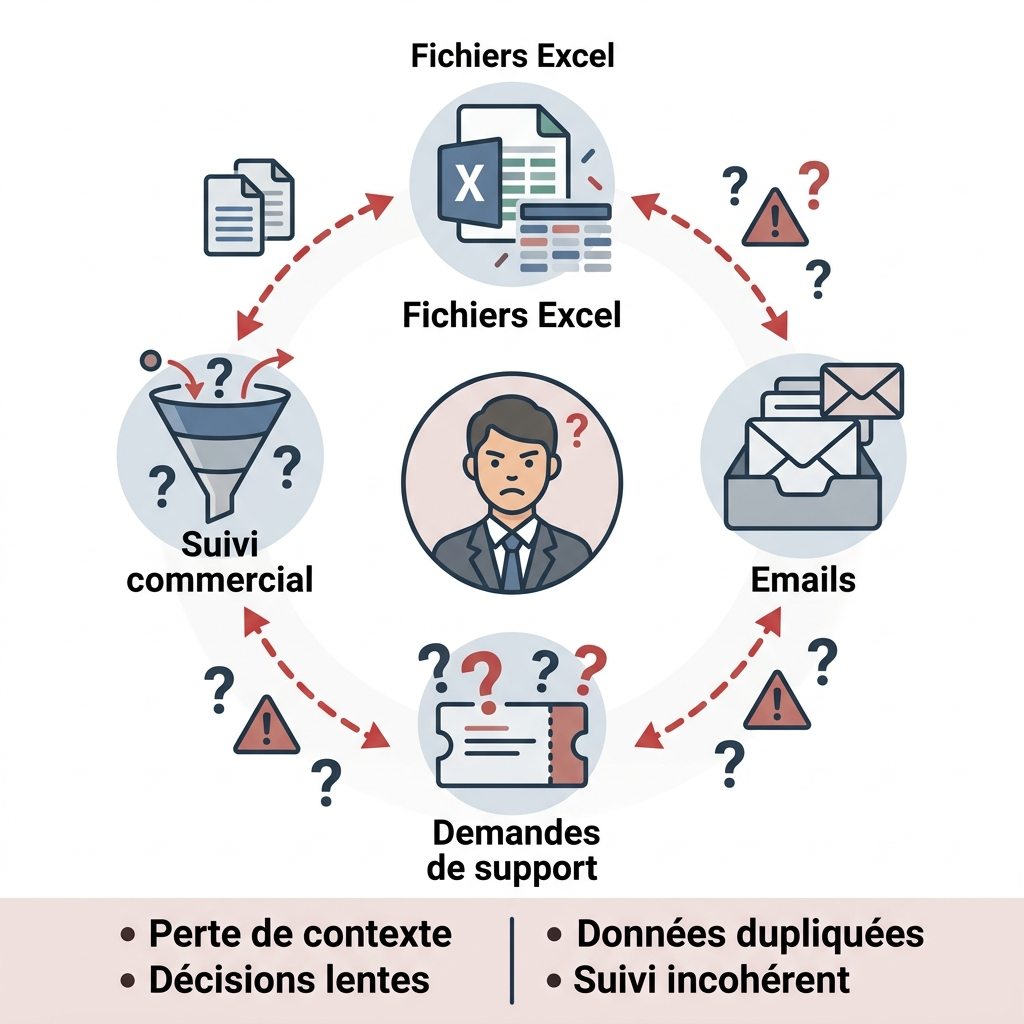
\includegraphics[width=0.72\textwidth]{dispersion_donnees.png}
    \caption{Impact d'une gestion dispersée de la relation client}
    \label{fig:problematique}
\end{figure}

\section{Présentation de l'organisme d'accueil}

\textbf{FRS} (\textit{FRS --- IT Development Company}) est une société de services et d'ingénierie informatique installée à Tunis. L'entreprise intervient dans la conception et le développement de solutions logicielles sur mesure, l'intégration de services numériques, l'accompagnement applicatif et le support technique. Son positionnement repose sur une proximité métier avec ses clients et sur la capacité à proposer des solutions adaptées plutôt que des outils génériques difficilement maîtrisables.\par
\vspace{0.3cm}

Le projet de stage s'inscrit dans cette logique. Il vise à doter l'entreprise d'un système unifié de suivi commercial et de support, capable de servir à la fois les équipes internes et les clients externes, tout en restant suffisamment souple pour évoluer avec les besoins futurs.

\begin{table}[H]
\centering
\caption{Fiche signalétique de l'organisme d'accueil}
\label{tab:fiche_entreprise}
\begin{tabularx}{0.95\textwidth}{|l|X|}
\hline
\textbf{Raison sociale} & FRS --- IT Development Company \\
\hline
\textbf{Secteur d'activité} & Services et ingénierie informatique, développement logiciel sur mesure \\
\hline
\textbf{Siège} & Tunis, Tunisie \\
\hline
\textbf{Année de création} & 2018 \\
\hline
\textbf{Site web} & \url{www.frs.tn} \\
\hline
\textbf{Effectif} & Environ 25 à 50 collaborateurs \\
\hline
\textbf{Services principaux} & Développement web et mobile, API et backend, solutions cloud, support applicatif, accompagnement numérique \\
\hline
\end{tabularx}
\end{table}

\begin{figure}[H]
    \centering
    
\includegraphics[width=6cm]{FRS_logo.jpg}
    \caption{Logo de l'entreprise FRS}
    \label{fig:logo_entreprise}
\end{figure}

\section{Problématique}
L'analyse du contexte a mis en évidence un ensemble de besoins convergents. L'entreprise a besoin d'un outil unique pour structurer la prospection, transformer les opportunités commerciales en dossiers clients exploitables, suivre les interactions de support et offrir aux clients un canal de consultation autonome.\par
\vspace{0.3cm}

La problématique peut être résumée ainsi : \textit{comment concevoir une plateforme CRM cohérente, sécurisée et évolutive, capable de centraliser les données commerciales et support, tout en proposant une expérience adaptée aux utilisateurs internes et aux clients externes ?}\par
\vspace{0.3cm}

Plus précisément, les difficultés à résoudre sont les suivantes :
\begin{enumerate}
    \item absence d'un référentiel unique pour les leads, comptes, contacts et opportunités ;
    \item manque de continuité entre la qualification d'un prospect et sa transformation en client suivi ;
    \item faible structuration du support client et de l'historique des échanges ;
    \item absence de portail client pour la consultation des tickets et des devis ;
    \item visibilité insuffisante sur les indicateurs de vente et de support ;
    \item absence de journal d'audit pour tracer les actions sensibles ;
    \item accès difficile à l'information métier et documentaire en situation de travail.
\end{enumerate}

\section{Approche proposée}
Pour répondre à cette problématique, une approche en plusieurs composantes a été retenue. L'idée n'est pas de produire une simple interface de gestion, mais un écosystème cohérent articulant les besoins internes, l'accès client et l'assistance informationnelle.

\begin{table}[H]
\centering
\caption{Composantes fonctionnelles de la solution proposée}
\label{tab:volets}
\begin{tabularx}{\textwidth}{|l|X|}
\hline
\textbf{Composante} & \textbf{Rôle dans la solution} \\
\hline
CRM web interne & Gestion des données commerciales et support par les équipes internes : leads, comptes, contacts, deals, devis, tickets, activités, utilisateurs, audit et reporting \\
\hline
Portail client web & Consultation sécurisée des tickets, messages, devis et informations de profil par les clients \\
\hline
Application mobile client & Accès nomade aux principales fonctions du portail client : tableau de bord, tickets, devis, profil et assistant conversationnel \\
\hline
Assistant conversationnel & Accès guidé à l'information métier à partir d'une base documentaire RAG regroupant présentation, services, FAQ, conditions générales, support et références projets \\
\hline
\end{tabularx}
\end{table}

\subsection{Fonctionnalités du CRM Web}
Le CRM web constitue le coeur fonctionnel du projet. Il rassemble les modules nécessaires au pilotage commercial et au traitement du support dans une même application :
\begin{itemize}
    \item authentification, gestion du profil et contrôle d'accès par rôles ;
    \item gestion des leads avec qualification et conversion ;
    \item gestion des comptes clients et des contacts associés ;
    \item pilotage du pipeline commercial et des devis ;
    \item gestion des tickets, des échanges publics et des notes internes ;
    \item suivi des activités commerciales et journalisation des actions ;
    \item tableaux de bord de vente et de support ;
    \item administration des utilisateurs et consultation de l'audit.
\end{itemize}

\subsection{Fonctionnalités de l'Application Mobile}
L'application mobile n'a pas vocation à reproduire l'ensemble du CRM interne. Elle est conçue comme une extension du portail client, orientée consultation et interaction :
\begin{itemize}
    \item connexion sécurisée pour les utilisateurs de rôle \texttt{client} ;
    \item consultation du tableau de bord client ;
    \item suivi et création de tickets ;
    \item consultation des devis liés au compte client ;
    \item accès à un assistant conversationnel pour obtenir des informations documentaires ;
    \item consultation et mise à jour du profil.
\end{itemize}

\subsection{Fonctionnalités du Chatbot IA}
Le module d'assistance s'appuie sur une logique documentaire. Il ne remplace pas les modules CRM, mais vient compléter le système en facilitant l'accès aux informations métier :
\begin{itemize}
    \item réponse en langage naturel à partir d'une base documentaire structurée ;
    \item interrogation de contenus liés à l'entreprise, aux services, à la FAQ et au support ;
    \item restitution d'une réponse contextualisée accompagnée de sources ;
    \item intégration dans le portail client web et dans l'application mobile ;
    \item fonctionnement dégradé possible lorsque le LLM externe n'est pas configuré.
\end{itemize}

\section{Méthodologie}

\subsection{Méthodologie Agile Scrum}
Le déroulement du projet a été structuré selon une logique \textbf{Agile Scrum}. Ce choix méthodologique permet d'avancer par itérations successives, de clarifier les objectifs à court terme et de réduire le risque de dérive entre le besoin exprimé et la solution développée. Chaque sprint est associé à un ensemble d'objectifs précis, depuis l'analyse jusqu'à la stabilisation finale du produit.

\begin{figure}[H]
    \centering
    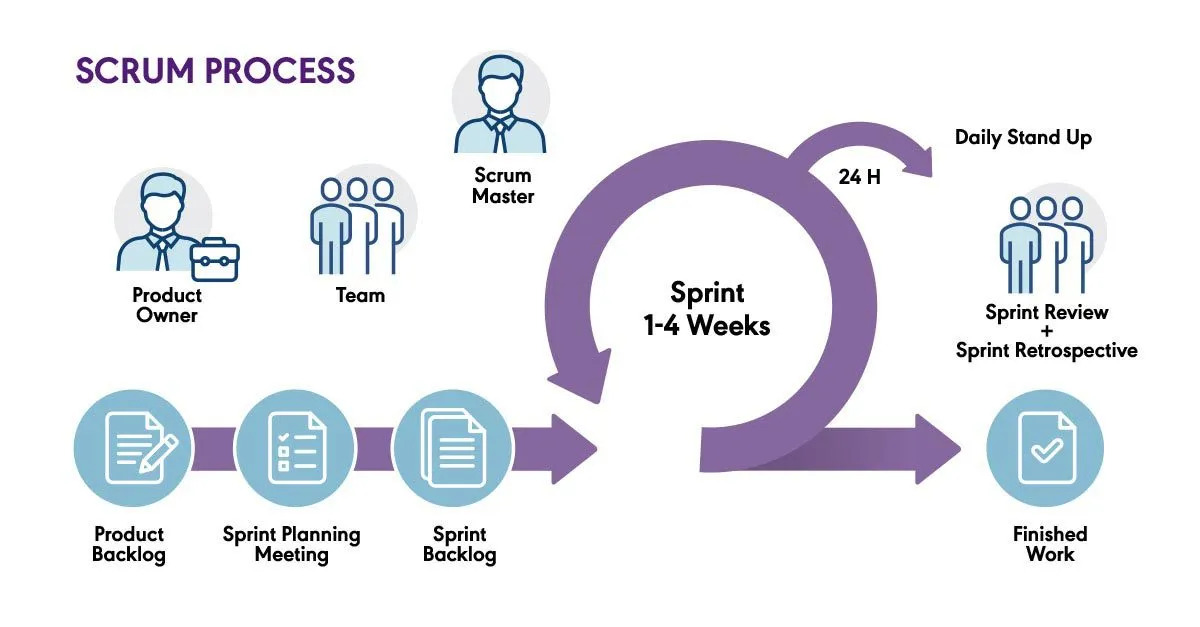
\includegraphics[width=0.7\textwidth]{scrum.png}
    \caption{Cycle général de la méthodologie Scrum}
    \label{fig:scrum}
\end{figure}

\subsection{Méthodologie CRISP-DM}
Pour le volet documentaire et conversationnel, une adaptation légère de la démarche \textbf{CRISP-DM} a été mobilisée. Elle a servi à structurer la sélection des documents, leur préparation, leur découpage, leur indexation et leur validation avant intégration dans la chaîne RAG. L'objectif n'était pas de réaliser un projet complet de data mining, mais d'utiliser une démarche méthodique pour constituer une base de connaissances exploitable et cohérente.

\begin{figure}[H]
    \centering
    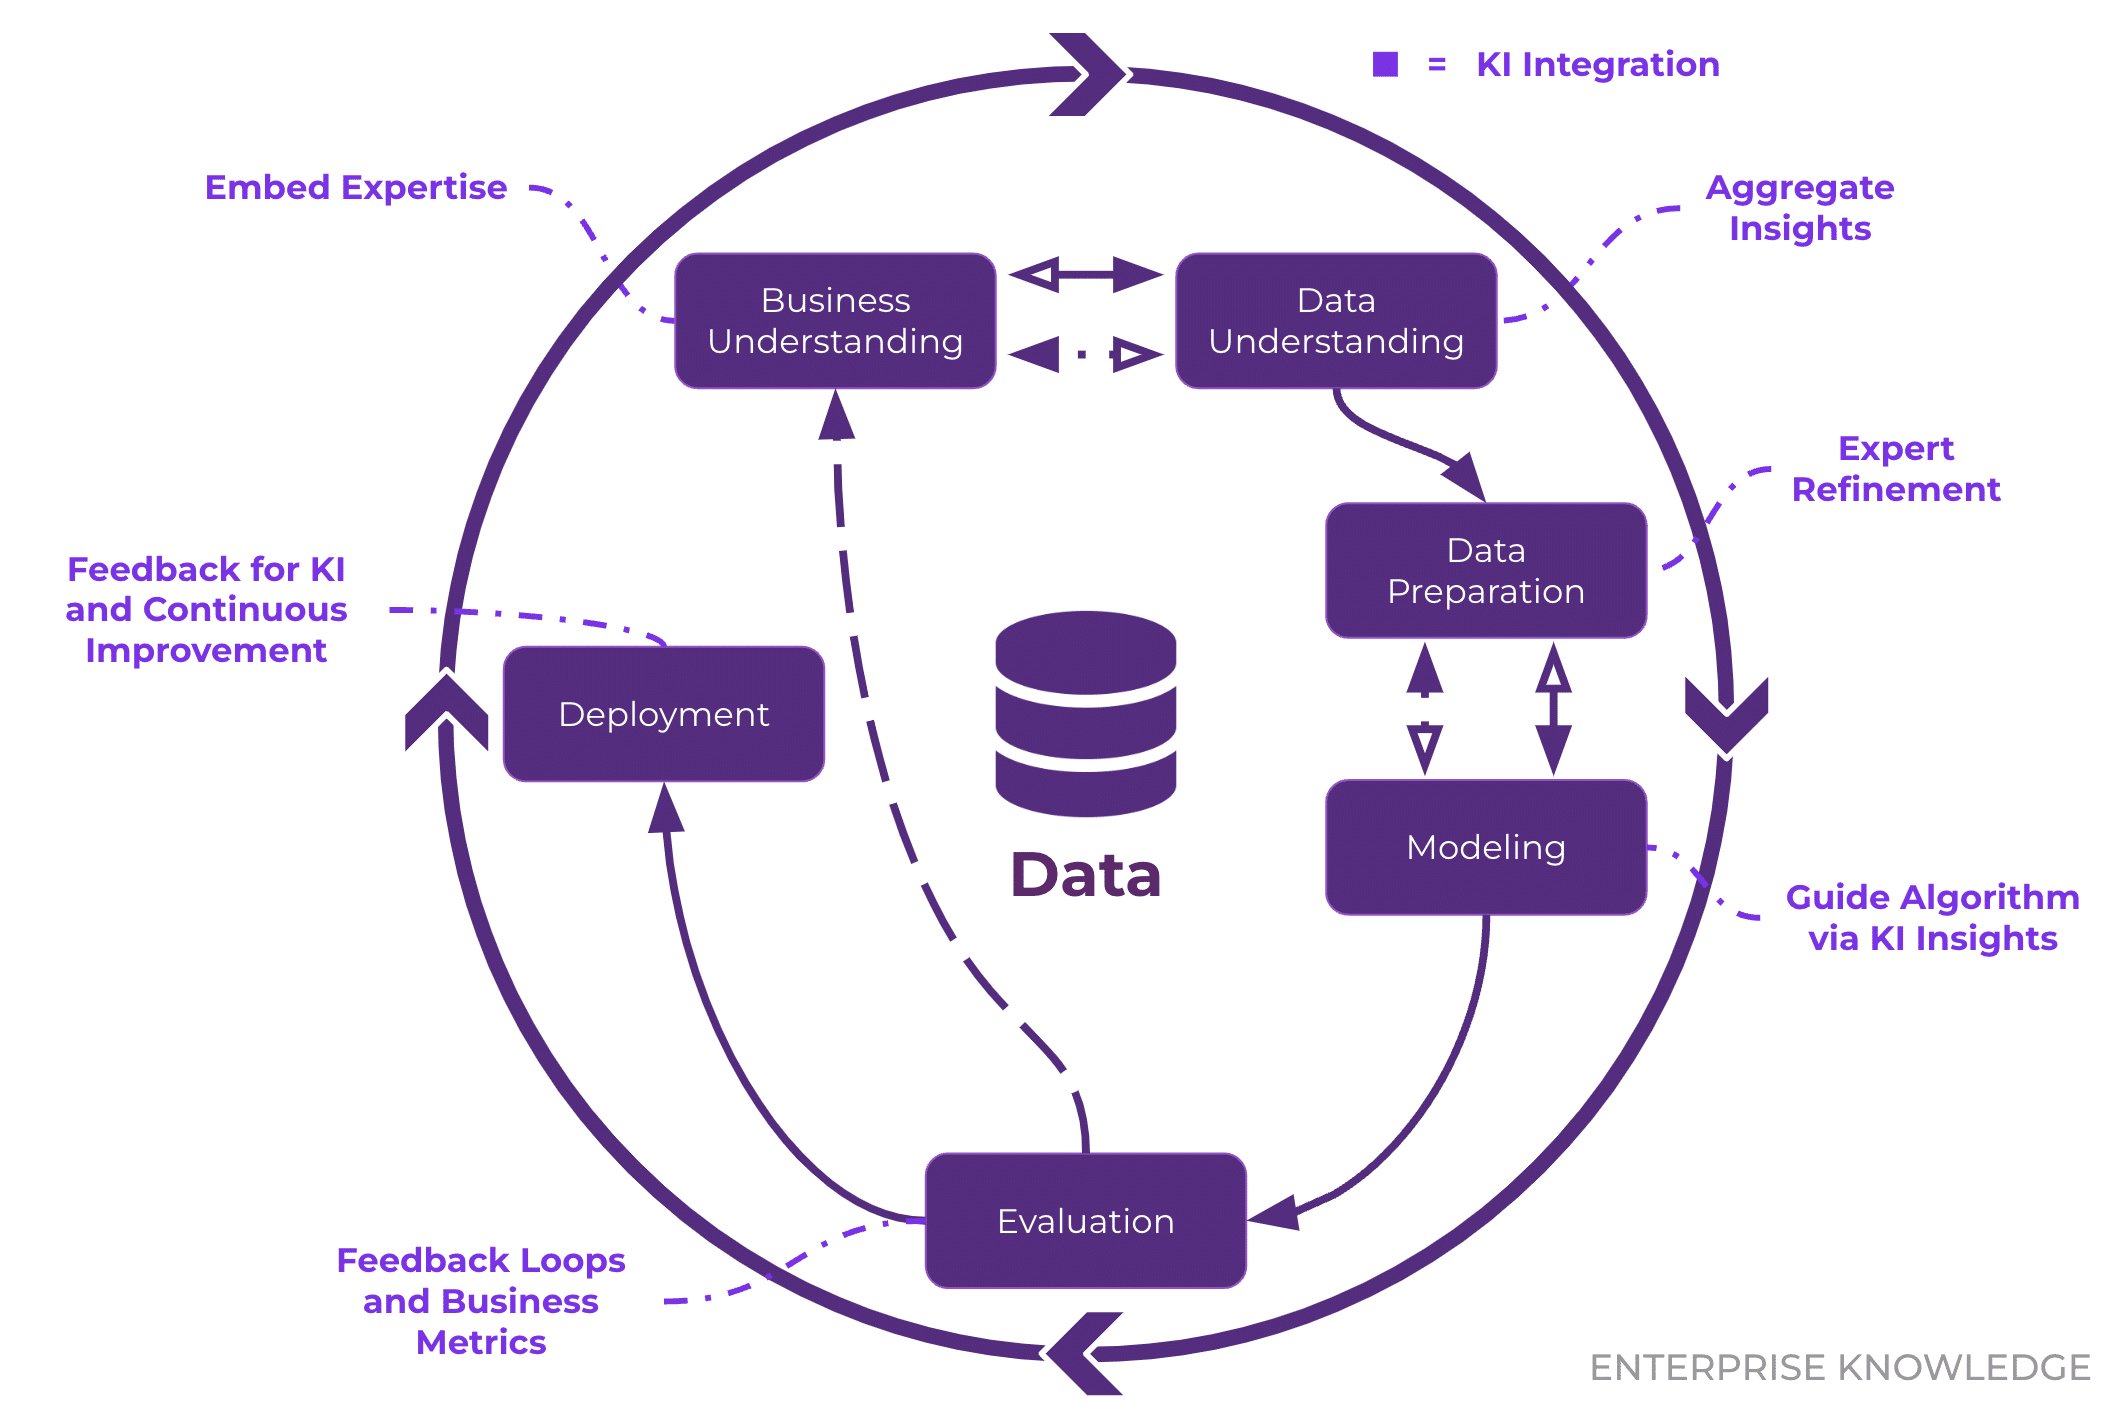
\includegraphics[width=0.4\textwidth]{crisp_dm.png}
    \caption{Cycle CRISP-DM mobilisé pour la préparation de la base documentaire}
    \label{fig:crisp_dm}
\end{figure}

\subsection{Organisation en sprints}
L'organisation temporelle du projet a été répartie en quatre sprints successifs, chacun associé à une finalité clairement identifiée.

\begin{table}[H]
\centering
\caption{Organisation du projet en sprints}
\label{tab:sprints}
\begin{tabularx}{\textwidth}{|c|X|c|}
\hline
\textbf{Sprint} & \textbf{Finalité principale} & \textbf{Durée} \\
\hline
Sprint 01 & Étude préalable, analyse des besoins, identification des acteurs et élaboration du backlog & 2 semaines \\
\hline
Sprint 02 & Conception UML, modélisation des données, architecture technique et conception de l'API & 2 semaines \\
\hline
Sprint 03 & Réalisation du backend, du frontend, du portail client, du mobile et du module d'assistance & 2 semaines \\
\hline
Sprint 04 & Validation fonctionnelle, revue RBAC, corrections de stabilisation et préparation du déploiement local & 2 semaines \\
\hline
\end{tabularx}
\end{table}

\section{Architecture globale}
L'architecture retenue s'appuie sur une logique \textbf{trois tiers} enrichie par des composants périphériques. Les interfaces web et mobile communiquent avec une API centralisée exposée par le backend FastAPI. Cette API accède à la base relationnelle MySQL pour les données métier, sollicite une base vectorielle locale pour l'assistant documentaire, et peut déclencher des notifications email via SMTP. Le frontend web est servi par Nginx dans une configuration intégrée à Docker Compose.\par
\vspace{0.3cm}

Cette organisation présente plusieurs avantages :
\begin{itemize}
    \item séparation claire entre présentation, logique métier et persistance ;
    \item réutilisation d'une même API par le web, le portail client et le mobile ;
    \item facilité de déploiement local grâce à la conteneurisation ;
    \item possibilité d'étendre ultérieurement le système par de nouveaux modules ou services.
\end{itemize}

\begin{figure}[H]
    \centering
    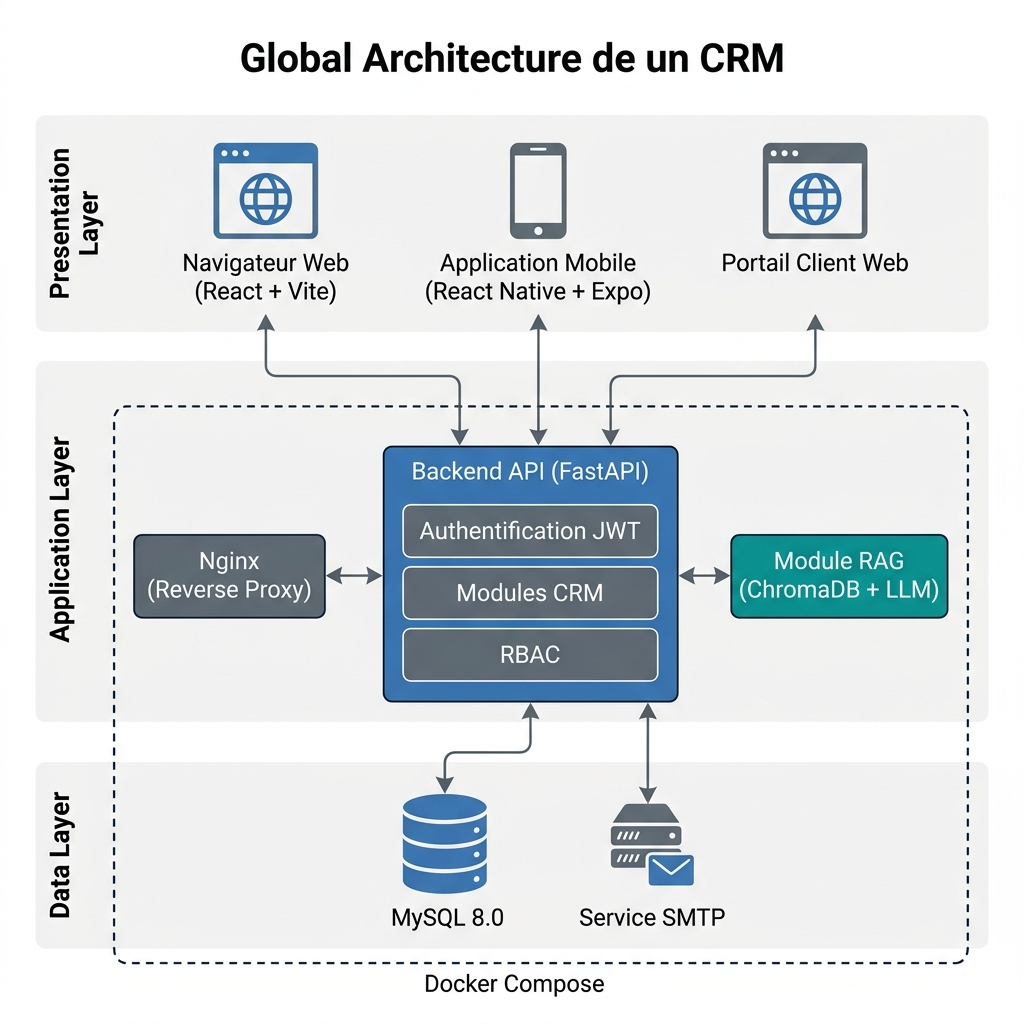
\includegraphics[width=0.78\textwidth]{architecture_globale.png}
    \caption{Architecture globale du système CRM}
    \label{fig:architecture}
\end{figure}

La planification temporelle de notre projet est réalisée selon la méthode de Gantt, comme illustré dans le Tableau 1.4. Elle met en évidence les différentes phases du projet, à savoir l’analyse et le recueil des besoins, la conception UML et l’architecture, le développement des composantes, ainsi que les étapes de validation, de test et de stabilisation, jusqu’à la rédaction du rapport final.
\begin{table}[H]
\centering
\caption{Planification simplifiée du projet}
\label{tab:gantt}
\begin{tabularx}{\textwidth}{|l|c|c|c|c|c|c|c|c|}
\hline
\textbf{Phase} & \textbf{S1} & \textbf{S2} & \textbf{S3} & \textbf{S4} & \textbf{S5} & \textbf{S6} & \textbf{S7} & \textbf{S8} \\
\hline
Analyse et recueil des besoins & $\bullet$ & $\bullet$ & & & & & & \\
\hline
Conception UML et architecture & & & $\bullet$ & $\bullet$ & & & & \\
\hline
Développement des composantes & & & & & $\bullet$ & $\bullet$ & & \\
\hline
Validation, tests et stabilisation & & & & & & & $\bullet$ & $\bullet$ \\
\hline
Rédaction du rapport & & & & & & & $\bullet$ & $\bullet$ \\
\hline
\end{tabularx}
\end{table}

\section{Environnement technique}
L'environnement technique du projet a été sélectionné de manière à concilier rapidité de développement, lisibilité du code et cohérence d'intégration entre les différentes couches du système.

\begin{table}[H]
\centering
\caption{Environnement technique du projet}
\label{tab:techno}
\begin{tabularx}{\textwidth}{|l|l|X|}
\hline
\textbf{Catégorie} & \textbf{Technologie} & \textbf{Utilisation dans le projet} \\
\hline
Frontend web & React 19 + Vite & Construction de l'application SPA interne et du portail client web \\
\hline
Frontend web & Tailwind CSS + composants Radix UI & Mise en forme de l'interface, composants réutilisables et cohérence visuelle \\
\hline
Frontend web & Axios + i18next & Appels API, intercepteurs d'authentification et support multilingue FR/EN \\
\hline
Mobile & React Native + Expo & Développement de l'application mobile client multiplateforme \\
\hline
Mobile & React Navigation + Expo Secure Store & Navigation mobile et stockage sécurisé du jeton JWT \\
\hline
Backend & FastAPI & Exposition de l'API REST et structuration des routes métier \\
\hline
Backend & SQLAlchemy + Pydantic & Mapping ORM, validation des schémas et sérialisation des données \\
\hline
Sécurité & JWT + bcrypt/passlib & Authentification, vérification des mots de passe et contrôle d'accès RBAC \\
\hline
Base de données & MySQL 8.0 & Stockage relationnel des données métier du CRM \\
\hline
Assistant documentaire & ChromaDB + LLM Groq optionnel & Indexation vectorielle locale et génération de réponses contextualisées \\
\hline
Infrastructure & Docker Compose + Nginx & Orchestration locale, reverse proxy frontend et exécution conteneurisée \\
\hline
Tests & Pytest, Vitest, Jest & Validation backend, frontend et mobile \\
\hline
Outils de développement & Git + Visual Studio Code & Gestion de version et environnement de développement \\
\hline
\end{tabularx}
\end{table}

\section{Conclusion}
Ce chapitre a permis de situer le projet dans son contexte métier, d'identifier la problématique à résoudre et de présenter les grandes lignes de la solution proposée. Il a également clarifié l'organisation méthodologique, l'architecture globale et l'environnement technique mobilisé. Ces éléments constituent la base de l'analyse détaillée menée dans le chapitre suivant.


% SPRINT 01 — Étude préalable et analyse
\newpage
\thispagestyle{empty}
\vspace*{\fill}
\begin{center}
\rule{0.8\textwidth}{0.5pt}

\vspace{1cm}
{\Huge\bfseries Sprint 01}

\vspace{0.5cm}
{\LARGE Étude Préalable et Analyse}
\vspace{1cm}

\rule{0.8\textwidth}{0.5pt}
\end{center}
\vspace*{\fill}
\newpage

\chapter{Sprint 01 : Étude Préalable et Analyse}
\minitoc
\newpage

\section{Introduction}
Le premier sprint a été consacré à la compréhension du besoin, à l'étude de l'existant et à la structuration fonctionnelle du futur système. Cette phase est essentielle, car elle conditionne la qualité des choix de conception et limite les risques d'écart entre la solution développée et les attentes métier.

\section{Objectifs du Sprint}
\begin{itemize}
    \item analyser les limites des pratiques actuelles et des solutions CRM du marché ;
    \item identifier les acteurs impliqués dans le système ;
    \item formaliser les besoins fonctionnels et non fonctionnels ;
    \item modéliser les cas d'utilisation principaux ;
    \item établir un backlog produit pour planifier les réalisations.
\end{itemize}

\section{Étude de l'existant}

\subsection{Analyse des solutions CRM existantes}
L'étude préalable a porté à la fois sur les outils utilisés habituellement par les entreprises de services et sur les solutions CRM généralistes disponibles sur le marché. Les plateformes majeures proposent des fonctionnalités avancées, mais elles s'accompagnent souvent d'un coût élevé, d'une logique de paramétrage complexe et d'une dépendance forte à un écosystème externe.\par
\vspace{0.3cm}

Dans le cadre de \textbf{FRS}, l'objectif n'était pas de concurrencer ces plateformes sur tous les plans, mais de concevoir une solution ciblée, réellement adaptée au cycle de vente, au support et à la relation client de l'entreprise.

\begin{table}[H]
\centering
\caption{Comparaison synthétique entre solutions existantes et solution développée}
\label{tab:comparaison_crm}
\begin{tabularx}{\textwidth}{|l|X|X|X|}
\hline
\textbf{Critère} & \textbf{Salesforce} & \textbf{HubSpot} & \textbf{Solution développée} \\
\hline
Coût d'adoption & Élevé à très élevé & Modèle freemium puis abonnements croissants & Maîtrisé par l'entreprise, adaptable au contexte de démonstration ou de déploiement local \\
\hline
Personnalisation métier & Forte mais souvent complexe & Moyenne selon les offres & Totale au niveau du code, des rôles et des flux métier \\
\hline
Portail client spécifique & Souvent optionnel ou additionnel & Partiel selon les modules & Intégré nativement au projet \\
\hline
Maîtrise des données & Hébergement externe & Hébergement externe & Déploiement local conteneurisé possible \\
\hline
Intégration d'une assistance documentaire & Services additionnels & Variable selon l'offre & Module RAG intégré à la solution \\
\hline
Adéquation à un projet pédagogique ou expérimental & Faible & Moyenne & Très forte \\
\hline
\end{tabularx}
\end{table}

\subsection{Critique de l'existant}
L'analyse a mis en évidence plusieurs limites dans les approches existantes ou dans les pratiques dispersées habituellement observées :
\begin{itemize}
    \item centralisation insuffisante des informations commerciales ;
    \item difficulté à relier la prospection, la négociation et le support dans un même référentiel ;
    \item faible visibilité sur l'historique des interactions ;
    \item absence d'un portail autonome pour les clients ;
    \item coût élevé des solutions génériques lorsqu'un fort niveau de personnalisation est requis.
\end{itemize}

\section{Identification des acteurs}
Le système CRM fait intervenir cinq acteurs principaux. Chacun dispose d'un périmètre fonctionnel distinct, ce qui justifie la mise en place d'une gestion des rôles et des permissions côté serveur.

\begin{table}[H]
\centering
\caption{Acteurs du système et responsabilités associées}
\label{tab:acteurs}
\begin{tabularx}{\textwidth}{|l|l|X|}
\hline
\textbf{Acteur} & \textbf{Rôle technique} & \textbf{Responsabilités principales} \\
\hline
Administrateur & \texttt{admin} & Administration du système, création des utilisateurs, supervision globale, accès à l'audit et aux fonctions sensibles \\
\hline
Manager & \texttt{manager} & Supervision des équipes, lecture des rapports, suivi des indicateurs et contrôle des activités clés \\
\hline
Commercial & \texttt{commercial} & Prospection, qualification des leads, gestion des comptes, des contacts, des deals et des devis \\
\hline
Support & \texttt{support} & Traitement des tickets, réponses aux clients, suivi des échanges et gestion opérationnelle du helpdesk \\
\hline
Client & \texttt{client} & Accès au portail et au mobile pour consulter les devis, créer ou suivre les tickets, échanger avec le support et utiliser l'assistant documentaire \\
\hline
\end{tabularx}
\end{table}

\section{Analyse des besoins fonctionnels}
Les besoins fonctionnels ont été regroupés par domaines métier afin de faciliter la future conception du système. Cette structuration reflète directement les modules observés dans le backend et les parcours disponibles dans les interfaces.

\subsection{Module Authentification et Sécurité}
Le système doit garantir un accès sécurisé aux interfaces et une séparation claire des droits d'utilisation :
\begin{itemize}
    \item authentification par email et mot de passe ;
    \item émission d'un jeton JWT pour sécuriser les appels à l'API ;
    \item gestion des rôles \texttt{admin}, \texttt{manager}, \texttt{commercial}, \texttt{support} et \texttt{client} ;
    \item consultation et mise à jour du profil utilisateur ;
    \item redirection vers l'espace adapté selon le rôle.
\end{itemize}

\subsection{Module Leads (Prospects)}
Le module leads doit couvrir le cycle de qualification commerciale :
\begin{itemize}
    \item création et mise à jour de fiches prospects ;
    \item suivi des statuts \textit{new}, \textit{contacted}, \textit{qualified}, \textit{unqualified} et \textit{converted} ;
    \item filtrage par source, statut, responsable et recherche textuelle ;
    \item conversion d'un lead qualifié en compte, contact et opportunité commerciale.
\end{itemize}

\subsection{Module Accounts (Comptes Clients)}
Le compte client représente l'entité pivot des relations commerciales et support :
\begin{itemize}
    \item centralisation des informations d'entreprise ;
    \item rattachement aux contacts, deals et tickets ;
    \item visibilité transversale pour les équipes commerciales et support ;
    \item administration des fiches comptes par les rôles internes.
\end{itemize}

\subsection{Module Contacts (Personnes)}
Le système doit permettre de gérer les interlocuteurs liés aux entreprises clientes :
\begin{itemize}
    \item création et modification des contacts ;
    \item rattachement obligatoire à un compte ;
    \item recherche par identité, coordonnées et société liée ;
    \item conservation des informations de poste et de contexte métier.
\end{itemize}

\subsection{Module Deals (Pipeline Commercial)}
Le pipeline commercial doit fournir une vision opérationnelle des opportunités :
\begin{itemize}
    \item gestion des opportunités par compte ;
    \item suivi des étapes \textit{qualification}, \textit{proposal}, \textit{negotiation}, \textit{won} et \textit{lost} ;
    \item mise à jour des montants, probabilités et dates de clôture ;
    \item journalisation des changements de stage.
\end{itemize}

\subsection{Module Quotes (Devis)}
Le module devis doit permettre de cadrer les propositions commerciales :
\begin{itemize}
    \item création de devis liés à un deal ;
    \item suivi des statuts \textit{draft}, \textit{sent}, \textit{accepted} et \textit{rejected} ;
    \item conservation de la référence, du montant et du support PDF éventuel ;
    \item notification du client lors de la création d'un nouveau devis.
\end{itemize}

\subsection{Module Tickets (Helpdesk)}
Le module support doit structurer le traitement des demandes clients :
\begin{itemize}
    \item création de tickets par les équipes internes ou par les clients via le portail ;
    \item suivi des priorités et des catégories ;
    \item gestion des statuts \textit{open}, \textit{in\_progress}, \textit{waiting\_customer}, \textit{resolved} et \textit{closed} ;
    \item messagerie associée avec distinction entre réponses publiques et notes internes ;
    \item assignation à des agents internes.
\end{itemize}

\subsection{Module Activities (Suivi Commercial)}
Le système doit conserver une trace des interactions commerciales significatives :
\begin{itemize}
    \item enregistrement d'appels, d'emails, de réunions ou de notes ;
    \item liaison aux comptes, contacts ou deals ;
    \item affichage chronologique des actions effectuées ;
    \item exploitation dans une logique de relance et de suivi commercial.
\end{itemize}

\subsection{Module Reporting et Audit}
Le projet doit offrir des fonctions d'analyse et de traçabilité :
\begin{itemize}
    \item indicateurs de vente : répartition des leads, pipeline, valeur gagnée, taux de conversion ;
    \item indicateurs support : tickets ouverts, tickets en retard, temps moyen de résolution ;
    \item audit des opérations sensibles pour conserver un historique exploitable.
\end{itemize}

\subsection{Module Portail Client}
Le portail client répond à un besoin fort d'autonomie et de transparence :
\begin{itemize}
    \item consultation des tickets et de leurs réponses publiques ;
    \item création de tickets depuis l'espace client ;
    \item consultation des devis liés au compte ;
    \item accès aux informations de profil ;
    \item isolement strict des données par compte client.
\end{itemize}

\subsection{Module Application Mobile}
L'application mobile reprend l'essentiel du portail client dans une logique d'usage nomade :
\begin{itemize}
    \item authentification client sécurisée ;
    \item tableau de bord synthétique ;
    \item suivi des tickets et ajout de messages ;
    \item consultation des devis ;
    \item accès à l'assistant documentaire ;
    \item message de blocage pour les rôles internes non prévus sur mobile.
\end{itemize}

\subsection{Module Chatbot IA (RAG)}
Le module d'assistance a pour objectif de faciliter l'accès à l'information métier et documentaire :
\begin{itemize}
    \item interrogation en langage naturel de documents d'entreprise ;
    \item restitution d'une réponse synthétique et contextualisée ;
    \item affichage des sources utilisées pour construire la réponse ;
    \item fonctionnement même en mode dégradé lorsque le fournisseur LLM n'est pas disponible.
\end{itemize}

\section{Besoins non fonctionnels}
Au-delà des fonctionnalités, le système doit respecter plusieurs exigences transverses qui influencent directement les choix techniques.

\begin{table}[H]
\centering
\caption{Principaux besoins non fonctionnels}
\label{tab:besoins_nf}
\begin{tabularx}{\textwidth}{|l|X|}
\hline
\textbf{Exigence} & \textbf{Description attendue} \\
\hline
Sécurité & Authentification robuste, contrôle d'accès par rôles, filtrage serveur des données visibles par chaque profil \\
\hline
Maintenabilité & Structuration modulaire du code, séparation des responsabilités et lisibilité des composants métier \\
\hline
Traçabilité & Journalisation des actions importantes pour faciliter la supervision et l'analyse postérieure \\
\hline
Portabilité & Possibilité d'exécuter localement le système et ses dépendances via Docker Compose \\
\hline
Ergonomie & Interfaces claires pour les usages internes et clients, adaptées au web et au mobile \\
\hline
Internationalisation & Support de plusieurs langues sur les interfaces web, avec une base FR/EN existante \\
\hline
Évolutivité & Capacité à ajouter de nouveaux modules, écrans ou sources documentaires sans remise à plat de l'architecture \\
\hline
\end{tabularx}
\end{table}

\section{Modélisation UML --- Diagrammes de cas d'utilisation}
Les diagrammes de cas d'utilisation permettent de relier les acteurs identifiés aux services attendus du système. Ils jouent un rôle important dans la clarification du périmètre fonctionnel avant le passage à la conception détaillée.

%% ─────────────────────────────────────────────────────────
%% 2.7.1  Diagramme de cas d'utilisation global
%% ─────────────────────────────────────────────────────────
\subsection{Diagramme de cas d'utilisation global}
Le diagramme global représente la vision d'ensemble du système avec ses cinq acteurs et ses principaux blocs fonctionnels. Chaque acteur est relié uniquement aux cas d'utilisation relevant de son périmètre de responsabilité.

\begin{figure}[H]
\centering
\resizebox{0.95\textwidth}{!}{%
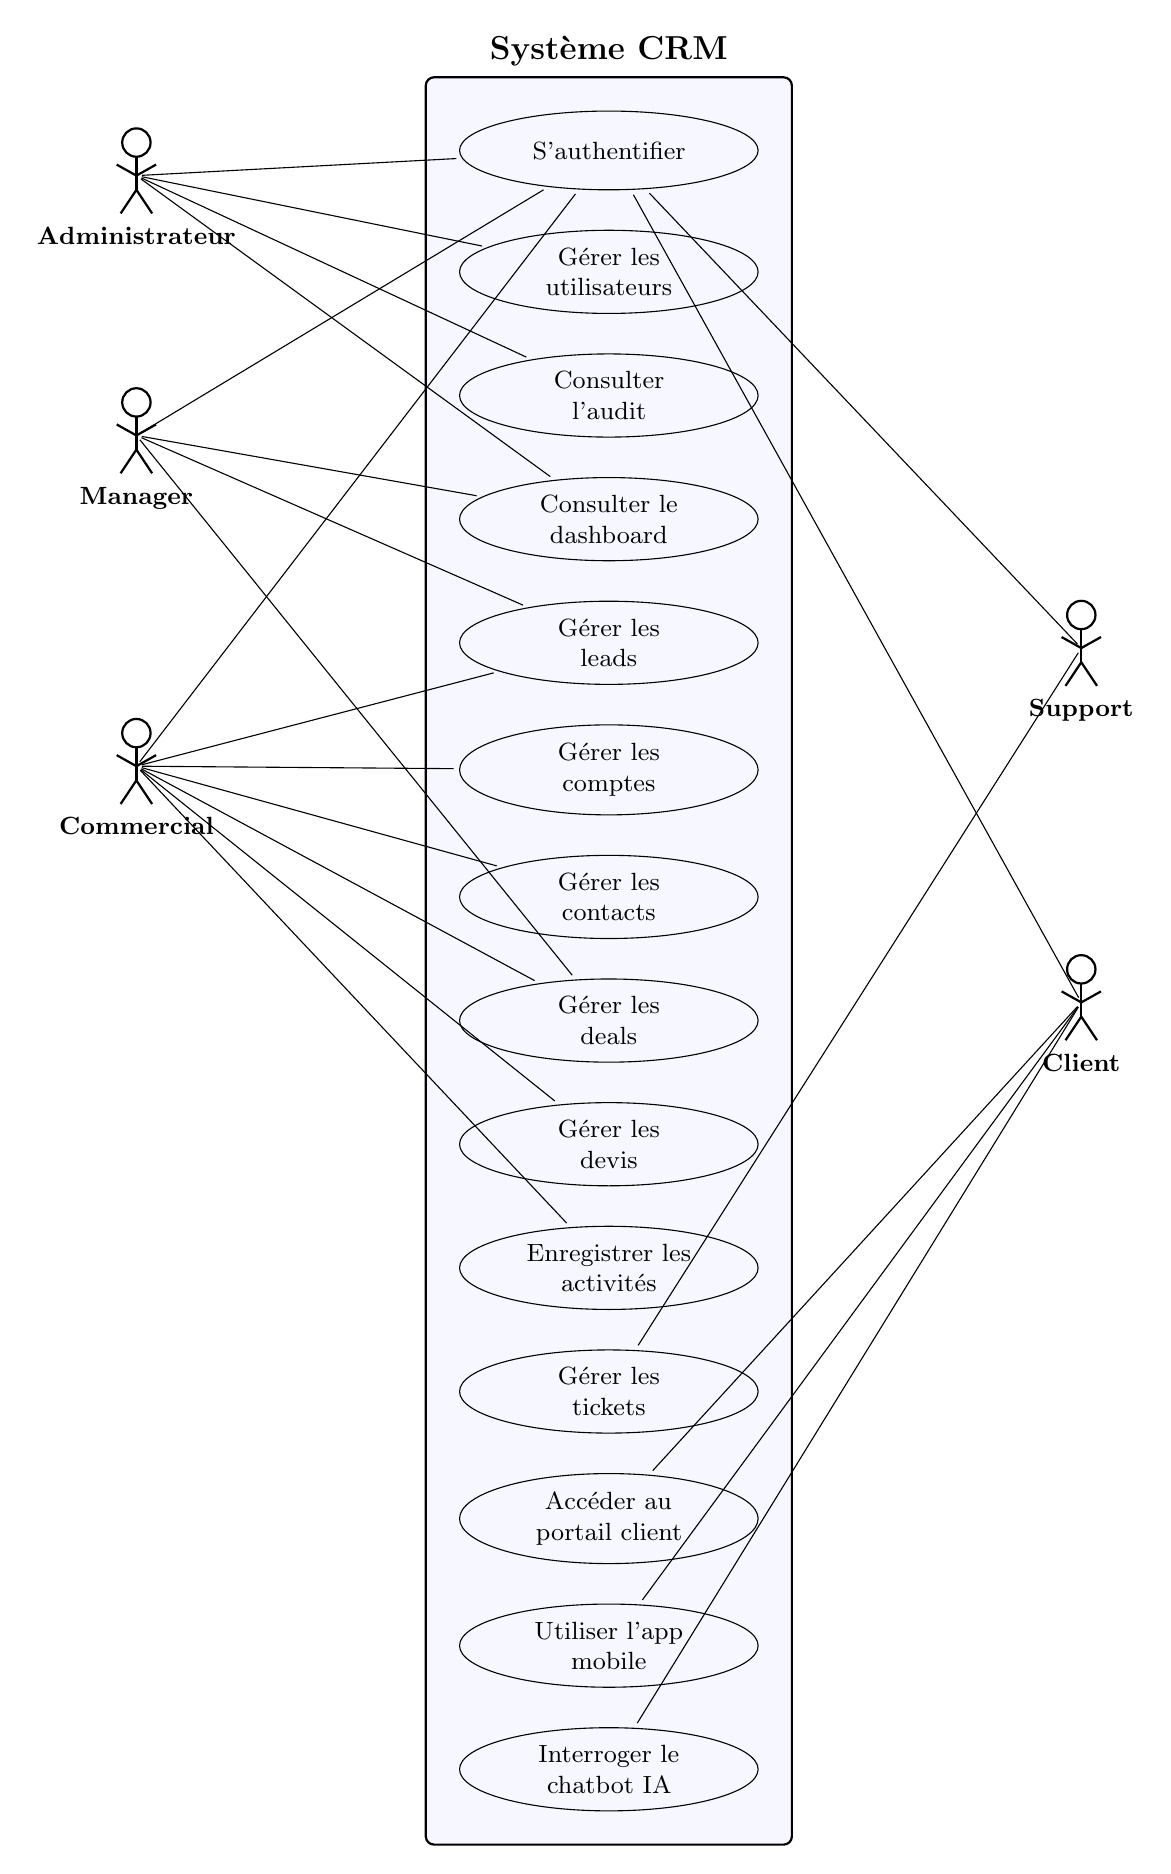
\begin{tikzpicture}[node distance=0.6cm and 1.2cm]

  %% ── Use cases ──
  \node[usecase] (auth)    {S'authentifier};
  \node[usecase, below=0.5cm of auth]  (users)   {Gérer les\\utilisateurs};
  \node[usecase, below=0.5cm of users] (audit)   {Consulter\\l'audit};
  \node[usecase, below=0.5cm of audit] (dash)    {Consulter le\\dashboard};
  \node[usecase, below=0.5cm of dash]  (leads)   {Gérer les\\leads};
  \node[usecase, below=0.5cm of leads] (accounts){Gérer les\\comptes};
  \node[usecase, below=0.5cm of accounts](contacts){Gérer les\\contacts};
  \node[usecase, below=0.5cm of contacts](deals) {Gérer les\\deals};
  \node[usecase, below=0.5cm of deals] (quotes)  {Gérer les\\devis};
  \node[usecase, below=0.5cm of quotes](activ)   {Enregistrer les\\activités};
  \node[usecase, below=0.5cm of activ] (tickets) {Gérer les\\tickets};
  \node[usecase, below=0.5cm of tickets](portail){Accéder au\\portail client};
  \node[usecase, below=0.5cm of portail](mobile) {Utiliser l'app\\mobile};
  \node[usecase, below=0.5cm of mobile](chatbot) {Interroger le\\chatbot IA};

  %% ── System boundary ──
  \begin{scope}[on background layer]
    \node[systemboundary, fit=(auth)(users)(audit)(dash)(leads)(accounts)
          (contacts)(deals)(quotes)(activ)(tickets)(portail)(mobile)(chatbot),
          label={[font=\large\bfseries]above:Système CRM}] (sys) {};
  \end{scope}

  %% ── Actors LEFT ──
  \umlactor{admin}{-6, -0.5}{Administrateur}
  \umlactor{manager}{-6, -3.8}{Manager}
  \umlactor{commercial}{-6, -8}{Commercial}

  %% ── Actors RIGHT ──
  \umlactor{support}{6, -6.5}{Support}
  \umlactor{client}{6, -11}{Client}

  %% ── Associations ──
  % Admin
  \draw[assoc] (admin) -- (auth);
  \draw[assoc] (admin) -- (users);
  \draw[assoc] (admin) -- (audit);
  \draw[assoc] (admin) -- (dash);

  % Manager
  \draw[assoc] (manager) -- (auth);
  \draw[assoc] (manager) -- (dash);
  \draw[assoc] (manager) -- (leads);
  \draw[assoc] (manager) -- (deals);

  % Commercial
  \draw[assoc] (commercial) -- (auth);
  \draw[assoc] (commercial) -- (leads);
  \draw[assoc] (commercial) -- (accounts);
  \draw[assoc] (commercial) -- (contacts);
  \draw[assoc] (commercial) -- (deals);
  \draw[assoc] (commercial) -- (quotes);
  \draw[assoc] (commercial) -- (activ);

  % Support
  \draw[assoc] (support) -- (auth);
  \draw[assoc] (support) -- (tickets);

  % Client
  \draw[assoc] (client) -- (auth);
  \draw[assoc] (client) -- (portail);
  \draw[assoc] (client) -- (mobile);
  \draw[assoc] (client) -- (chatbot);

\end{tikzpicture}%
}
\caption{Diagramme de cas d'utilisation global du système CRM}
\label{fig:uc_global}
\end{figure}

%% ─────────────────────────────────────────────────────────
%% 2.7.2  Cas d'utilisation — Gestion des Leads
%% ─────────────────────────────────────────────────────────
\subsection{Cas d'utilisation --- Gestion des Leads}
Ce diagramme met en évidence le cycle d'acquisition commerciale, de la création d'un lead jusqu'à sa conversion en compte, contact et deal.

\begin{figure}[H]
\centering
\resizebox{0.92\textwidth}{!}{%
\begin{tikzpicture}[node distance=0.55cm and 1cm]

  %% ── Use cases principaux ──
  \node[usecase] (creer)     {Créer un lead};
  \node[usecase, below=of creer]   (modifier)  {Modifier un lead};
  \node[usecase, below=of modifier](consulter) {Consulter les leads};
  \node[usecase, below=of consulter](filtrer)  {Filtrer les leads};
  \node[usecase, below=of filtrer] (qualifier) {Qualifier un lead};
  \node[usecase, below=of qualifier](convertir){Convertir un lead};
  \node[usecase, below=of convertir](supprimer){Supprimer un lead};

  %% ── Use cases inclus (conversion) ──
  \node[usecaseSmall, right=3cm of convertir, yshift=1.2cm]  (cAccount) {Créer un\\compte};
  \node[usecaseSmall, right=3cm of convertir]                (cContact) {Créer un\\contact};
  \node[usecaseSmall, right=3cm of convertir, yshift=-1.2cm] (cDeal)    {Créer un\\deal};

  %% ── System boundary ──
  \begin{scope}[on background layer]
    \node[systemboundary,
          fit=(creer)(modifier)(consulter)(filtrer)(qualifier)(convertir)(supprimer)
              (cAccount)(cContact)(cDeal),
          label={[font=\large\bfseries]above:Module Leads}] (sys) {};
  \end{scope}

  %% ── Actors ──
  \umlactor{commercial}{-5.5, -3.2}{Commercial}
  \umlactor{manager}{-5.5, -6.5}{Manager}

  %% ── Associations — Commercial ──
  \draw[assoc] (commercial) -- (creer);
  \draw[assoc] (commercial) -- (modifier);
  \draw[assoc] (commercial) -- (consulter);
  \draw[assoc] (commercial) -- (filtrer);
  \draw[assoc] (commercial) -- (qualifier);
  \draw[assoc] (commercial) -- (convertir);
  \draw[assoc] (commercial) -- (supprimer);

  %% ── Associations — Manager ──
  \draw[assoc] (manager) -- (consulter);
  \draw[assoc] (manager) -- (filtrer);

  %% ── Include arrows ──
  \draw[include] (convertir) -- node[above, font=\footnotesize, sloped] {\guillemotleft include\guillemotright} (cAccount);
  \draw[include] (convertir) -- node[above, font=\footnotesize, sloped] {\guillemotleft include\guillemotright} (cContact);
  \draw[include] (convertir) -- node[above, font=\footnotesize, sloped] {\guillemotleft include\guillemotright} (cDeal);

\end{tikzpicture}%
}
\caption{Cas d'utilisation du module Leads}
\label{fig:uc_leads}
\end{figure}

%% ─────────────────────────────────────────────────────────
%% 2.7.3  Cas d'utilisation — Gestion des Tickets
%% ─────────────────────────────────────────────────────────
\subsection{Cas d'utilisation --- Gestion des Tickets}
Le module support fait intervenir plusieurs interactions entre le client, les agents internes et les responsables de supervision.

\begin{figure}[H]
\centering
\resizebox{0.92\textwidth}{!}{%
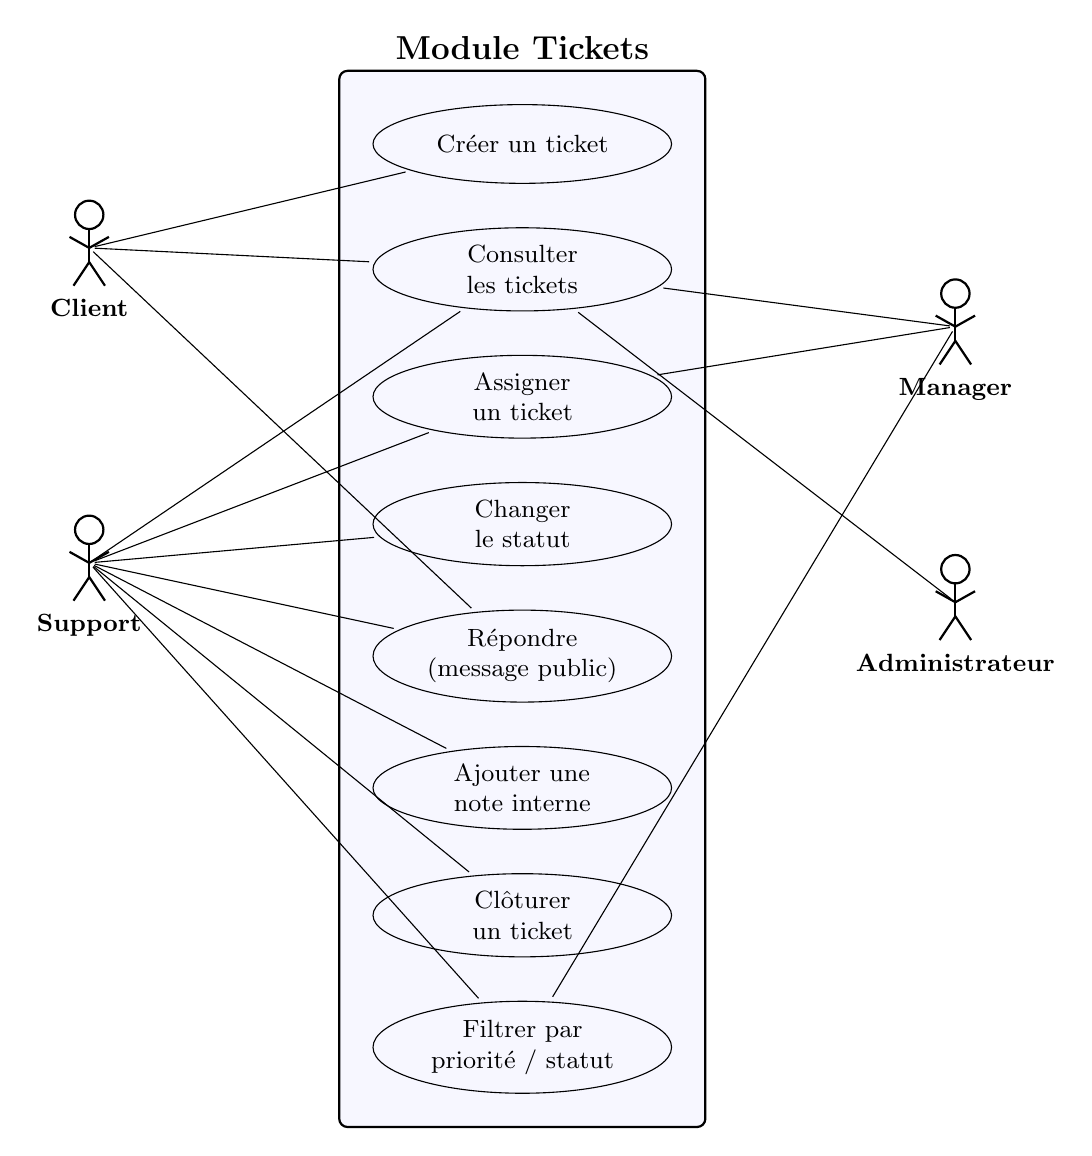
\begin{tikzpicture}[node distance=0.55cm and 1cm]

  %% ── Use cases ──
  \node[usecase] (creerT)   {Créer un ticket};
  \node[usecase, below=of creerT]   (consultT) {Consulter les tickets};
  \node[usecase, below=of consultT] (assignT)  {Assigner un ticket};
  \node[usecase, below=of assignT]  (statutT)  {Changer le statut};
  \node[usecase, below=of statutT]  (repondreT){Répondre\\(message public)};
  \node[usecase, below=of repondreT](noteT)    {Ajouter une\\note interne};
  \node[usecase, below=of noteT]    (cloreT)   {Clôturer un ticket};
  \node[usecase, below=of cloreT]   (filtrerT) {Filtrer par\\priorité / statut};

  %% ── System boundary ──
  \begin{scope}[on background layer]
    \node[systemboundary,
          fit=(creerT)(consultT)(assignT)(statutT)(repondreT)(noteT)(cloreT)(filtrerT),
          label={[font=\large\bfseries]above:Module Tickets}] (sys) {};
  \end{scope}

  %% ── Actors LEFT ──
  \umlactor{clientT}{-5.5, -1.5}{Client}
  \umlactor{supportT}{-5.5, -5.5}{Support}

  %% ── Actors RIGHT ──
  \umlactor{managerT}{5.5, -2.5}{Manager}
  \umlactor{adminT}{5.5, -6}{Administrateur}

  %% ── Associations — Client ──
  \draw[assoc] (clientT) -- (creerT);
  \draw[assoc] (clientT) -- (consultT);
  \draw[assoc] (clientT) -- (repondreT);

  %% ── Associations — Support ──
  \draw[assoc] (supportT) -- (consultT);
  \draw[assoc] (supportT) -- (assignT);
  \draw[assoc] (supportT) -- (statutT);
  \draw[assoc] (supportT) -- (repondreT);
  \draw[assoc] (supportT) -- (noteT);
  \draw[assoc] (supportT) -- (cloreT);
  \draw[assoc] (supportT) -- (filtrerT);

  %% ── Associations — Manager ──
  \draw[assoc] (managerT) -- (consultT);
  \draw[assoc] (managerT) -- (assignT);
  \draw[assoc] (managerT) -- (filtrerT);

  %% ── Associations — Admin ──
  \draw[assoc] (adminT) -- (consultT);

\end{tikzpicture}%
}
\caption{Cas d'utilisation du module Tickets}
\label{fig:uc_tickets}
\end{figure}

%% ─────────────────────────────────────────────────────────
%% 2.7.4  Cas d'utilisation — Portail Client
%% ─────────────────────────────────────────────────────────
\subsection{Cas d'utilisation --- Portail Client}
Le portail client reste volontairement ciblé sur l'autonomie, la consultation et la communication avec le support.

\begin{figure}[H]
\centering
\resizebox{0.82\textwidth}{!}{%
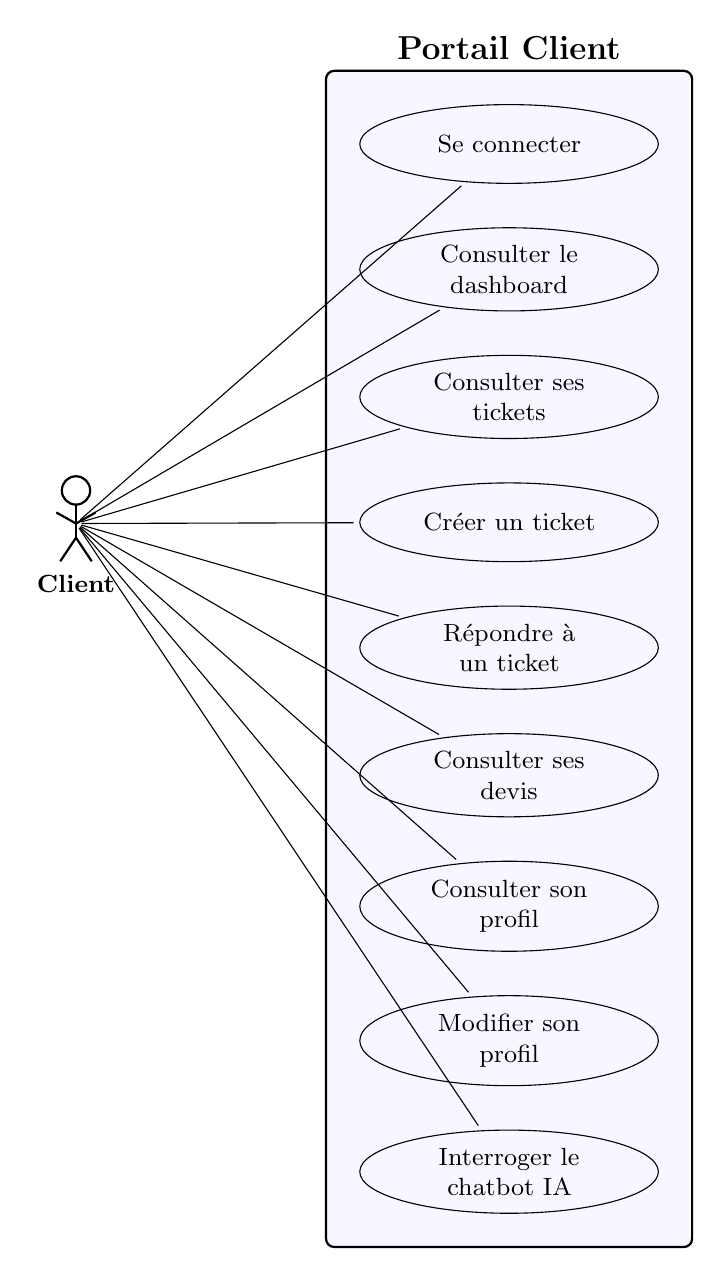
\begin{tikzpicture}[node distance=0.55cm and 1cm]

  %% ── Use cases ──
  \node[usecase] (connecter) {Se connecter};
  \node[usecase, below=of connecter] (dashP)    {Consulter le\\dashboard};
  \node[usecase, below=of dashP]     (ticketsP) {Consulter ses\\tickets};
  \node[usecase, below=of ticketsP]  (creerTP)  {Créer un ticket};
  \node[usecase, below=of creerTP]   (repondP)  {Répondre à\\un ticket};
  \node[usecase, below=of repondP]   (devisP)   {Consulter ses\\devis};
  \node[usecase, below=of devisP]    (profilP)  {Consulter son\\profil};
  \node[usecase, below=of profilP]   (modifP)   {Modifier son\\profil};
  \node[usecase, below=of modifP]    (chatP)    {Interroger le\\chatbot IA};

  %% ── System boundary ──
  \begin{scope}[on background layer]
    \node[systemboundary,
          fit=(connecter)(dashP)(ticketsP)(creerTP)(repondP)(devisP)(profilP)(modifP)(chatP),
          label={[font=\large\bfseries]above:Portail Client}] (sys) {};
  \end{scope}

  %% ── Actor ──
  \umlactor{clientP}{-5.5, -5}{Client}

  %% ── Associations ──
  \draw[assoc] (clientP) -- (connecter);
  \draw[assoc] (clientP) -- (dashP);
  \draw[assoc] (clientP) -- (ticketsP);
  \draw[assoc] (clientP) -- (creerTP);
  \draw[assoc] (clientP) -- (repondP);
  \draw[assoc] (clientP) -- (devisP);
  \draw[assoc] (clientP) -- (profilP);
  \draw[assoc] (clientP) -- (modifP);
  \draw[assoc] (clientP) -- (chatP);

\end{tikzpicture}%
}
\caption{Cas d'utilisation du portail client}
\label{fig:uc_portail}
\end{figure}

%% ─────────────────────────────────────────────────────────
%% 2.7.5  Cas d'utilisation — Application Mobile
%% ─────────────────────────────────────────────────────────
\subsection{Cas d'utilisation --- Application Mobile}
L'application mobile prolonge les usages du portail client dans un contexte d'accès nomade. Les rôles internes reçoivent un message de blocage les invitant à utiliser l'interface web.

\begin{figure}[H]
\centering
\resizebox{0.88\textwidth}{!}{%
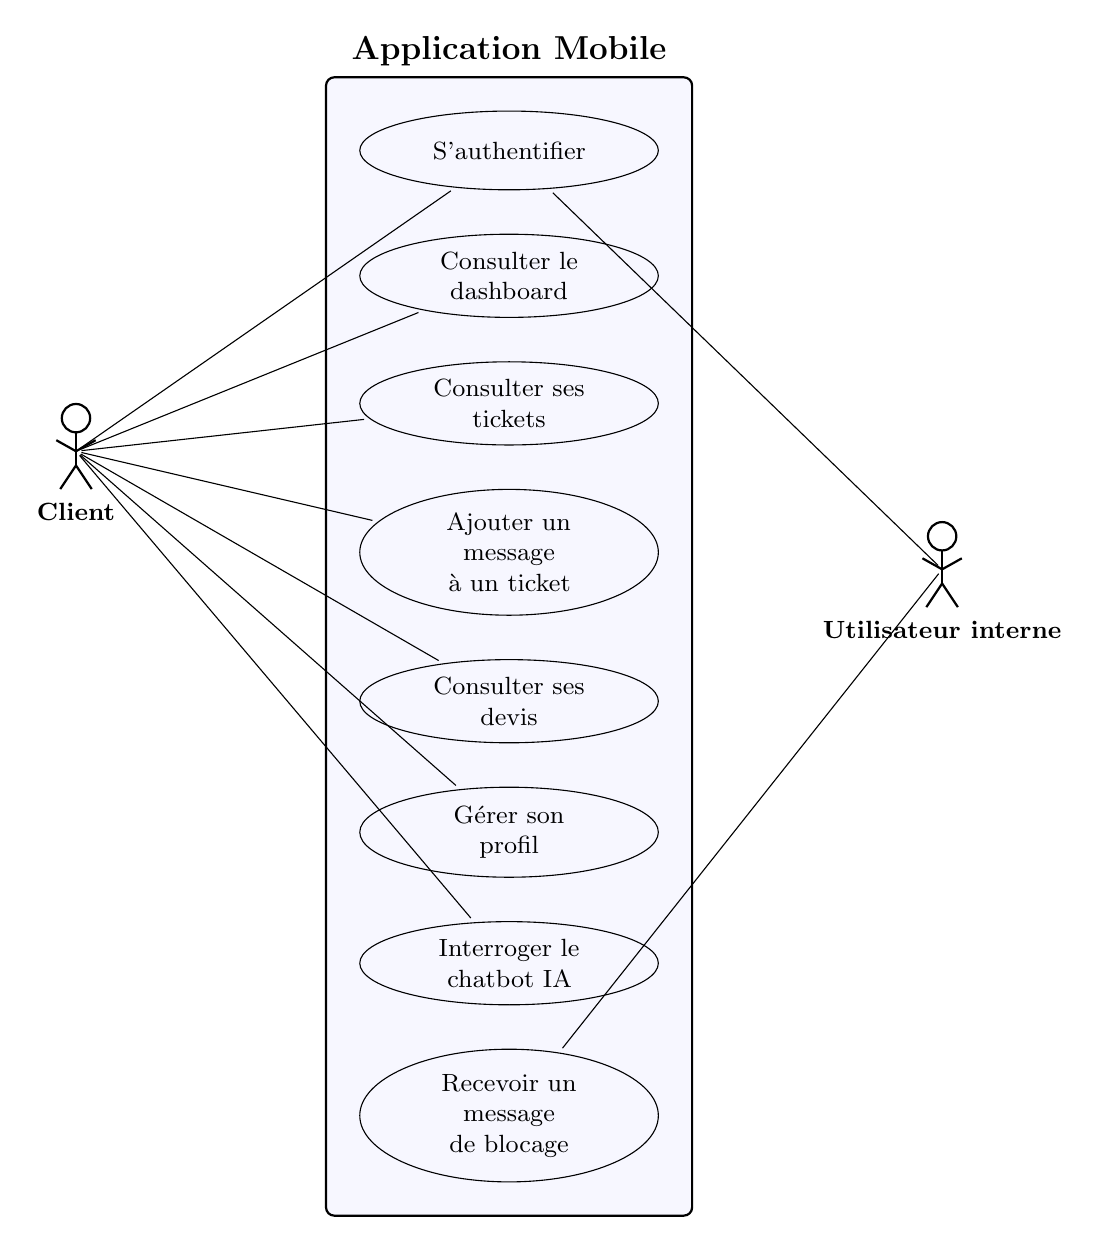
\begin{tikzpicture}[node distance=0.55cm and 1cm]

  %% ── Use cases ──
  \node[usecase] (authM)    {S'authentifier};
  \node[usecase, below=of authM]    (dashM)    {Consulter le\\dashboard};
  \node[usecase, below=of dashM]    (ticketsM) {Consulter ses\\tickets};
  \node[usecase, below=of ticketsM] (msgM)     {Ajouter un message\\à un ticket};
  \node[usecase, below=of msgM]     (devisM)   {Consulter ses\\devis};
  \node[usecase, below=of devisM]   (profilM)  {Gérer son\\profil};
  \node[usecase, below=of profilM]  (chatM)    {Interroger le\\chatbot IA};
  \node[usecase, below=of chatM]    (blocM)    {Recevoir un\\message de blocage};

  %% ── System boundary ──
  \begin{scope}[on background layer]
    \node[systemboundary,
          fit=(authM)(dashM)(ticketsM)(msgM)(devisM)(profilM)(chatM)(blocM),
          label={[font=\large\bfseries]above:Application Mobile}] (sys) {};
  \end{scope}

  %% ── Actors ──
  \umlactor{clientM}{-5.5, -4}{Client}
  \umlactor{intM}{5.5, -5.5}{Utilisateur interne}

  %% ── Associations — Client ──
  \draw[assoc] (clientM) -- (authM);
  \draw[assoc] (clientM) -- (dashM);
  \draw[assoc] (clientM) -- (ticketsM);
  \draw[assoc] (clientM) -- (msgM);
  \draw[assoc] (clientM) -- (devisM);
  \draw[assoc] (clientM) -- (profilM);
  \draw[assoc] (clientM) -- (chatM);

  %% ── Associations — Utilisateur interne ──
  \draw[assoc] (intM) -- (authM);
  \draw[assoc] (intM) -- (blocM);

\end{tikzpicture}%
}
\caption{Cas d'utilisation de l'application mobile}
\label{fig:uc_mobile}
\end{figure}

%% ─────────────────────────────────────────────────────────
%% 2.7.6  Cas d'utilisation — Chatbot IA (RAG)
%% ─────────────────────────────────────────────────────────
\subsection{Cas d'utilisation --- Chatbot IA}
Le module d'assistance peut être représenté comme un service transverse permettant à l'utilisateur authentifié d'interroger la base documentaire et d'obtenir une réponse contextualisée.

\begin{figure}[H]
\centering
\resizebox{0.88\textwidth}{!}{%
\begin{tikzpicture}[node distance=0.7cm and 1.2cm]

  %% ── Use cases ──
  \node[usecase] (question) {Poser une question\\en langage naturel};
  \node[usecase, below right=1cm and 3cm of question] (recherche) {Rechercher dans\\la base documentaire};
  \node[usecase, below=1cm of recherche] (reponse) {Générer une réponse\\contextualisée};
  \node[usecase, below=1cm of reponse]   (sources) {Afficher les\\sources utilisées};
  \node[usecase, right=2.5cm of reponse]   (degrade) {Gérer le mode\\dégradé};

  %% ── System boundary ──
  \begin{scope}[on background layer]
    \node[systemboundary,
          fit=(question)(recherche)(reponse)(sources)(degrade),
          label={[font=\large\bfseries]above:Module Chatbot IA (RAG)}] (sys) {};
  \end{scope}

  %% ── Actors ──
  \umlactor{userC}{-5.5, -1}{Utilisateur authentifié}

  %% ── Actor système (rectangle) ──
  \node[draw, rectangle, minimum width=1.6cm, minimum height=1.2cm,
        font=\small\bfseries, align=center] (rag) at (12, -3.5) {Système\\RAG};

  %% ── Associations ──
  \draw[assoc] (userC) -- (question);

  %% ── Include arrows ──
  \draw[include] (question) -- node[above, font=\footnotesize, sloped] {\guillemotleft include\guillemotright} (recherche);
  \draw[include] (recherche) -- node[right, font=\footnotesize] {\guillemotleft include\guillemotright} (reponse);
  \draw[include] (reponse) -- node[right, font=\footnotesize] {\guillemotleft include\guillemotright} (sources);

  %% ── Extend arrow ──
  \draw[extend] (degrade) -- node[above, font=\footnotesize, sloped] {\guillemotleft extend\guillemotright} (reponse);

  %% ── Système RAG associations ──
  \draw[assoc] (rag) -- (recherche);
  \draw[assoc] (rag) -- (reponse);

\end{tikzpicture}%
}
\caption{Cas d'utilisation du chatbot documentaire (RAG)}
\label{fig:uc_chatbot}
\end{figure}

\section{Backlog produit}
Le backlog suivant synthétise les besoins prioritaires identifiés au terme de l'analyse. Il a servi de base à la planification des sprints techniques.

\begin{table}[H]
\centering
\footnotesize
\caption{Backlog produit synthétique}
\label{tab:backlog}
\begin{tabularx}{\textwidth}{|c|X|c|c|}
\hline
\textbf{ID} & \textbf{User Story} & \textbf{Priorité} & \textbf{Sprint cible} \\
\hline
US01 & En tant que commercial, je veux créer, qualifier et suivre un lead afin d'organiser la prospection & Haute & Sprint 03 \\
\hline
US02 & En tant que commercial, je veux convertir un lead qualifié en compte, contact et deal afin de réduire la ressaisie & Haute & Sprint 03 \\
\hline
US03 & En tant que commercial ou manager, je veux piloter le pipeline des deals pour suivre la maturité des opportunités & Haute & Sprint 03 \\
\hline
US04 & En tant que support, je veux gérer des tickets avec réponses publiques et notes internes afin de structurer le helpdesk & Haute & Sprint 03 \\
\hline
US05 & En tant que client, je veux consulter mes tickets et mes devis dans un portail dédié afin de gagner en autonomie & Haute & Sprint 03 \\
\hline
US06 & En tant qu'administrateur, je veux gérer les utilisateurs et les rôles afin de sécuriser l'accès au système & Haute & Sprint 03 \\
\hline
US07 & En tant que manager, je veux consulter des indicateurs de vente et de support afin de piloter l'activité & Haute & Sprint 03 \\
\hline
US08 & En tant qu'utilisateur interne, je veux enregistrer des activités commerciales afin de conserver l'historique des interactions & Moyenne & Sprint 03 \\
\hline
US09 & En tant que client, je veux accéder à mon espace depuis un mobile afin de suivre mes demandes en mobilité & Moyenne & Sprint 03 \\
\hline
US10 & En tant qu'utilisateur authentifié, je veux interroger la base documentaire via un assistant conversationnel afin d'obtenir rapidement une information métier & Moyenne & Sprint 03 \\
\hline
\end{tabularx}
\end{table}

\section{Résultats du Sprint}
\begin{table}[H]
\centering
\caption{Livrables du Sprint 01}
\label{tab:livrables_s1}
\begin{tabularx}{\textwidth}{|X|c|}
\hline
\textbf{Livrable} & \textbf{Statut} \\
\hline
Étude comparative et critique de l'existant & $\checkmark$ \\
\hline
Identification des acteurs et des responsabilités & $\checkmark$ \\
\hline
Formalisation des besoins fonctionnels et non fonctionnels & $\checkmark$ \\
\hline
Préparation des cas d'utilisation du système & $\checkmark$ \\
\hline
Élaboration d'un backlog produit structuré & $\checkmark$ \\
\hline
\end{tabularx}
\end{table}

\section{Conclusion}
Le premier sprint a permis de poser les fondations du projet. L'étude de l'existant a justifié la pertinence d'une solution sur mesure, l'identification des acteurs a clarifié le périmètre d'utilisation, et l'analyse des besoins a fourni un cadre précis pour la conception détaillée. Le chapitre suivant s'appuie sur ces résultats pour présenter les modèles, les diagrammes et l'architecture de la solution.


% SPRINT 02 — Conception du système CRM
\newpage
\thispagestyle{empty}
\vspace*{\fill}
\begin{center}
\rule{0.8\textwidth}{0.5pt}

\vspace{1cm}
{\Huge\bfseries Sprint 02}

\vspace{0.5cm}
{\LARGE Conception du Système CRM}
\vspace{1cm}

\rule{0.8\textwidth}{0.5pt}
\end{center}
\vspace*{\fill}
\newpage

\chapter{Sprint 02 : Conception du Système CRM}
\minitoc
\newpage

\section{Introduction}
Ce chapitre présente le deuxième sprint, consacré à la conception détaillée du système. À partir des besoins identifiés précédemment, il s'agit ici de structurer les modèles métier, de préciser le schéma de données, de décrire les flux critiques du système et de définir une architecture capable de supporter les interfaces web, client, mobile et documentaire.

\section{Objectifs du Sprint}
\begin{itemize}
    \item modéliser les entités métier et leurs relations ;
    \item élaborer le schéma relationnel de la base de données ;
    \item formaliser les séquences de fonctionnement essentielles ;
    \item définir l'architecture technique du backend, du frontend, du mobile et du module RAG ;
    \item spécifier les principaux endpoints de l'API REST.
\end{itemize}

\section{Diagramme de classes}
Le diagramme de classes permet de représenter les objets métiers manipulés par le système ainsi que leurs liens. Dans le cas du CRM réalisé, la modélisation tourne autour de deux grands axes : le cycle commercial et le cycle de support. À ces deux axes s'ajoutent des éléments transverses comme l'utilisateur, les activités, l'audit et les rôles.

\begin{table}[H]
\centering
\caption{Entités principales du diagramme de classes}
\label{tab:classes}
\begin{tabularx}{\textwidth}{|l|X|}
\hline
\textbf{Classe métier} & \textbf{Rôle dans le système} \\
\hline
User & Représente un utilisateur authentifié du système, interne ou client, avec un rôle et un périmètre d'accès \\
\hline
Account & Porte les informations de l'entreprise cliente et sert d'entité pivot pour les contacts, deals et tickets \\
\hline
Contact & Représente l'interlocuteur rattaché à un compte client \\
\hline
Lead & Représente un prospect avant sa conversion en éléments structurés du CRM \\
\hline
Deal & Représente une opportunité commerciale suivie dans le pipeline \\
\hline
Quote & Représente un devis associé à une opportunité commerciale \\
\hline
Ticket & Représente une demande de support liée à un compte client \\
\hline
TicketMessage & Représente un message public ou une note interne dans le cycle de vie d'un ticket \\
\hline
Activity & Représente une interaction commerciale liée à un compte, un contact ou un deal \\
\hline
AuditLog & Conserve l'historique des opérations sensibles pour assurer la traçabilité \\
\hline
\end{tabularx}
\end{table}

\PlaceholderFigure{0.92\textwidth}{6.5cm}{Diagramme de classes du système CRM}{Espace réservé à l'insertion du diagramme de classes final, incluant les entités User, Account, Contact, Lead, Deal, Quote, Ticket, TicketMessage, Activity et AuditLog.}{fig:diag_classes}

\subsection{Relations entre entités}
Les relations entre classes structurent le comportement global du système. Les plus importantes sont résumées ci-dessous.

\begin{table}[H]
\centering
\caption{Principales relations métier du système}
\label{tab:relations_classes}
\begin{tabularx}{\textwidth}{|l|X|}
\hline
\textbf{Relation} & \textbf{Interprétation métier} \\
\hline
Account --- Contact & Un compte regroupe plusieurs interlocuteurs métiers \\
\hline
Account --- Deal & Une entreprise cliente peut faire l'objet de plusieurs opportunités commerciales \\
\hline
Deal --- Quote & Une opportunité peut donner lieu à plusieurs versions ou états de devis \\
\hline
Account --- Ticket & Les demandes de support sont rattachées à l'entreprise cliente concernée \\
\hline
Ticket --- TicketMessage & Chaque ticket conserve l'historique chronologique des échanges associés \\
\hline
Lead --- Account / Contact / Deal & La conversion d'un lead crée les entités commerciales structurées et mémorise les références correspondantes \\
\hline
User --- Account & Un utilisateur client peut être lié à un compte ; un utilisateur interne peut être propriétaire d'un compte, d'un deal ou d'un lead \\
\hline
Activity --- Account / Contact / Deal & Une activité commerciale peut être liée à une ou plusieurs entités métier suivies \\
\hline
AuditLog --- User & Chaque action auditée est rattachée, quand cela est possible, à son acteur \\
\hline
\end{tabularx}
\end{table}

\section{Diagramme Entité-Relation (ERD)}
Le schéma de base de données traduit le modèle objet en structure relationnelle. Le projet s'appuie sur une base \textbf{MySQL} contenant dix tables principales. Ces tables couvrent l'authentification, les objets métiers du cycle commercial, le helpdesk et l'audit. Les relations sont implémentées par des clés étrangères assurant la cohérence entre les comptes, les contacts, les deals, les devis, les tickets et les utilisateurs.\par
\vspace{0.3cm}

La conception du schéma a été pensée pour répondre à deux exigences : d'une part, conserver des relations simples à comprendre et à exploiter côté ORM ; d'autre part, permettre l'évolution des modules sans remettre en cause la structure générale du système.

\PlaceholderFigure{0.92\textwidth}{6.5cm}{Diagramme Entité-Relation de la base CRM}{Espace réservé à l'insertion du diagramme ERD final montrant les dix tables principales, leurs clés primaires, leurs clés étrangères et leurs cardinalités.}{fig:erd}

\section{Diagrammes de séquence}
Les diagrammes de séquence décrivent les interactions dynamiques entre les interfaces, l'API et les couches métier du backend. Ils mettent en évidence les étapes de traitement des scénarios critiques.

\subsection{Séquence --- Authentification JWT}
Le scénario d'authentification repose sur la soumission des identifiants, la vérification du mot de passe, la génération d'un jeton JWT et la récupération du profil courant. Ce flux conditionne l'accès à tous les autres modules du système.

\PlaceholderFigure{0.88\textwidth}{5.8cm}{Diagramme de séquence de l'authentification JWT}{Espace réservé à l'insertion du diagramme représentant l'utilisateur, l'interface cliente, l'API d'authentification, le service métier, la couche de sécurité et la base de données.}{fig:seq_auth}

\subsection{Séquence --- Conversion d'un Lead}
La conversion d'un lead est l'un des scénarios métier les plus importants. Elle illustre la manière dont une opération unique aboutit à la création de plusieurs entités corrélées : compte, contact et deal. Ce flux doit rester transactionnel et cohérent.

\PlaceholderFigure{0.9\textwidth}{5.8cm}{Diagramme de séquence de conversion d'un lead}{Espace réservé à l'insertion du diagramme montrant la récupération du lead qualifié, la création de l'Account, du Contact et du Deal, puis la mise à jour du statut du lead.}{fig:seq_conversion}

\subsection{Séquence --- Cycle de vie d'un Ticket}
Le traitement d'un ticket implique plusieurs participants : le client, le portail ou l'espace interne, l'API support, les services métier, la base de données et le système de notification. La séquence doit montrer la distinction entre message public et note interne ainsi que la mise à jour du statut du ticket.

\PlaceholderFigure{0.9\textwidth}{5.8cm}{Diagramme de séquence du cycle de vie d'un ticket}{Espace réservé à l'insertion du diagramme illustrant la création du ticket, l'assignation, l'ajout de messages, la notification du client et la résolution.}{fig:seq_ticket}

\subsection{Séquence --- Chatbot documentaire (RAG)}
Le flux du module d'assistance repose sur une logique documentaire : l'utilisateur soumet une question, le backend recherche les fragments les plus pertinents dans la base vectorielle, puis renvoie une réponse contextualisée avec ses sources. Le LLM externe intervient uniquement lorsqu'il est configuré ; sinon, le système retourne une réponse de secours basée sur la recherche locale.

\PlaceholderFigure{0.84\textwidth}{5.8cm}{Diagramme de séquence du chatbot documentaire}{Espace réservé à l'insertion du diagramme représentant l'utilisateur, l'API chatbot, la chaîne RAG, la base vectorielle ChromaDB et le fournisseur LLM optionnel.}{fig:seq_rag}

\section{Conception de l'architecture}

\subsection{Architecture backend --- FastAPI + organisation par domaines}
Le backend est conçu comme une API REST structurée par domaines métier. Chaque domaine rassemble les modèles, schémas, repositories et services correspondant à une responsabilité fonctionnelle précise. Cette organisation facilite la lisibilité, limite le couplage et rend les évolutions plus prévisibles.

\begin{table}[H]
\centering
\caption{Organisation logique du backend}
\label{tab:arch_backend}
\begin{tabularx}{\textwidth}{|l|X|X|}
\hline
\textbf{Couche} & \textbf{Responsabilité} & \textbf{Exemples dans le projet} \\
\hline
API & Exposer les endpoints, valider les dépendances et orchestrer les services & routeurs \texttt{auth}, \texttt{leads}, \texttt{tickets}, \texttt{client}, \texttt{chatbot}, \texttt{email} \\
\hline
Domaines métier & Encapsuler les règles métier et la logique applicative & services de conversion de lead, gestion des tickets, reporting, audit \\
\hline
Persistance & Accéder à la base relationnelle via l'ORM & repositories SQLAlchemy et modèles métier \\
\hline
Composants partagés & Fournir sécurité, pagination, exceptions et services transverses & JWT, pagination, email, base repository \\
\hline
Composants documentaires & Gérer l'indexation, la recherche et la génération de réponse documentaire & vector store, chaîne RAG, client LLM \\
\hline
\end{tabularx}
\end{table}

\subsection{Architecture frontend --- React SPA}
Le frontend web est pensé comme une application SPA séparant les parcours internes et les parcours clients. L'espace interne s'appuie sur un layout dédié pour les modules CRM, tandis que le portail client dispose de son propre layout et d'une logique de navigation distincte. La communication avec le backend est centralisée dans un service Axios, complété par un contexte d'authentification et un contexte de thème.\par
\vspace{0.3cm}

Cette séparation apporte plusieurs avantages :
\begin{itemize}
    \item clarté des parcours selon les profils ;
    \item réutilisation d'un même backend pour plusieurs interfaces ;
    \item mise en place de comportements transverses comme l'authentification, l'internationalisation et le mode sombre ;
    \item intégration d'un widget de chat documentaire dans l'espace client.
\end{itemize}

\subsection{Architecture mobile --- React Native}
L'application mobile reprend la logique du portail client dans un contexte natif léger. Elle repose sur une navigation de type \textbf{Native Stack}, sur un contexte d'authentification et sur un stockage sécurisé du jeton via \textbf{Expo Secure Store}. Le choix d'une application dédiée au rôle \texttt{client} simplifie les flux et limite les risques d'incohérence avec les parcours internes.

\begin{table}[H]
\centering
\caption{Principes de conception de l'application mobile}
\label{tab:arch_mobile}
\begin{tabularx}{\textwidth}{|l|X|}
\hline
\textbf{Bloc} & \textbf{Description} \\
\hline
Navigation & Enchaînement des écrans login, tableau de bord client, tickets, devis, chatbot et profil \\
\hline
Authentification & Gestion du jeton et récupération du profil via un contexte React Native \\
\hline
Sécurité locale & Stockage du jeton JWT dans Expo Secure Store \\
\hline
Services & Centralisation des appels API via Axios \\
\hline
Restriction métier & Blocage explicite des rôles internes, redirigés vers la version web \\
\hline
\end{tabularx}
\end{table}

\subsection{Architecture RAG --- Chatbot IA}
Le module d'assistance adopte une architecture documentaire simple et robuste :
\begin{enumerate}
    \item préparation d'un ensemble de documents métier rédigés en Markdown ;
    \item découpage de ces documents en fragments exploitables ;
    \item indexation de ces fragments dans une base vectorielle locale ;
    \item recherche des passages les plus pertinents pour une question donnée ;
    \item génération d'une réponse contextualisée à partir des résultats obtenus ;
    \item repli sur une réponse documentaire simplifiée lorsque le LLM externe n'est pas disponible.
\end{enumerate}

\PlaceholderFigure{0.86\textwidth}{5.8cm}{Architecture du module RAG}{Espace réservé à l'insertion du diagramme montrant les documents Markdown, l'indexation, ChromaDB, la recherche contextuelle, le LLM optionnel et la réponse finale.}{fig:arch_rag}

\subsection{Architecture Docker Compose}
Le projet est conçu pour être exécuté localement dans un environnement conteneurisé. La pile principale comprend une base de données MySQL, un backend FastAPI et un frontend servi par Nginx. Des services supplémentaires dédiés aux campagnes de test sont définis dans le fichier \texttt{docker-compose.yml}.

\begin{table}[H]
\centering
\caption{Services définis dans l'architecture Docker Compose}
\label{tab:docker_arch}
\begin{tabularx}{\textwidth}{|l|l|X|}
\hline
\textbf{Service} & \textbf{Port principal} & \textbf{Rôle} \\
\hline
\texttt{db} & 3307 sur l'hôte & Base MySQL du projet \\
\hline
\texttt{backend} & 8000 & API FastAPI et logique métier \\
\hline
\texttt{frontend} & 3000 & Application web servie via Nginx avec reverse proxy API \\
\hline
\texttt{backend\_unit\_tests} & --- & Exécution des tests unitaires backend \\
\hline
\texttt{backend\_integration\_tests} & --- & Exécution des tests d'intégration API \\
\hline
\texttt{frontend\_tests} & --- & Exécution des tests frontend \\
\hline
\texttt{mobile\_tests} & --- & Exécution des tests mobile \\
\hline
\end{tabularx}
\end{table}

\section{Conception de l'API REST}
La conception de l'API REST s'appuie sur une logique de routes métier versionnées en \texttt{/api/v1}. Les endpoints couvrent l'authentification, la gestion des entités commerciales, le helpdesk, le portail client, les rapports, les notifications email et le module d'assistance.

\begin{table}[H]
\centering
\footnotesize
\caption{Extrait des principaux endpoints de l'API REST}
\label{tab:api}
\begin{tabularx}{\textwidth}{|l|l|X|}
\hline
\textbf{Méthode} & \textbf{Endpoint} & \textbf{Description} \\
\hline
POST & /api/v1/auth/login & Authentification et retour d'un jeton JWT \\
\hline
GET & /api/v1/auth/me & Récupération du profil utilisateur connecté \\
\hline
GET / POST & /api/v1/leads & Consultation et création des leads \\
\hline
POST & /api/v1/leads/\{id\}/convert & Conversion d'un lead qualifié en compte, contact et deal \\
\hline
GET / POST & /api/v1/deals & Consultation et création des opportunités commerciales \\
\hline
PATCH & /api/v1/deals/\{id\}/stage & Mise à jour du stage d'un deal dans le pipeline \\
\hline
GET / POST & /api/v1/quotes & Consultation et création des devis \\
\hline
GET / POST & /api/v1/tickets/\{id\}/messages & Consultation et ajout de messages sur un ticket interne \\
\hline
GET & /api/v1/reports/sales & Indicateurs de performance commerciale \\
\hline
GET & /api/v1/reports/support & Indicateurs du support client \\
\hline
GET & /api/v1/reports/audit-logs & Consultation du journal d'audit \\
\hline
GET / POST & /api/v1/client/tickets & Consultation et création de tickets côté client \\
\hline
GET & /api/v1/client/quotes & Consultation des devis liés au compte client \\
\hline
POST & /api/v1/chatbot & Envoi d'une question au module d'assistance documentaire \\
\hline
GET & /api/v1/chatbot/status & Consultation de l'état du module RAG \\
\hline
GET / POST & /api/v1/email/... & Vérification et envoi de notifications email \\
\hline
\end{tabularx}
\end{table}

\section{Résultats du Sprint}
\begin{table}[H]
\centering
\caption{Livrables du Sprint 02}
\label{tab:livrables_s2}
\begin{tabularx}{\textwidth}{|X|c|}
\hline
\textbf{Livrable} & \textbf{Statut} \\
\hline
Modèle de classes métier et relations principales & $\checkmark$ \\
\hline
Schéma relationnel et principes ERD & $\checkmark$ \\
\hline
Séquences des scénarios critiques & $\checkmark$ \\
\hline
Architecture technique backend, frontend, mobile et RAG & $\checkmark$ \\
\hline
Spécification synthétique de l'API REST & $\checkmark$ \\
\hline
\end{tabularx}
\end{table}

\section{Conclusion}
Le deuxième sprint a permis de transformer les besoins du chapitre précédent en une vision structurée de la solution. Les modèles de données, les flux dynamiques et l'architecture technique sont désormais clarifiés. Cette conception sert de référence pour la phase suivante, consacrée à la réalisation concrète des différentes composantes du système.


% SPRINT 03 — Réalisation technique
\newpage
\thispagestyle{empty}
\vspace*{\fill}
\begin{center}
\rule{0.8\textwidth}{0.5pt}

\vspace{1cm}
{\Huge\bfseries Sprint 03}

\vspace{0.5cm}
{\LARGE Réalisation Technique}
\vspace{1cm}

\rule{0.8\textwidth}{0.5pt}
\end{center}
\vspace*{\fill}
\newpage

\chapter{Sprint 03 : Réalisation Technique}
\minitoc
\newpage

\section{Introduction}
Ce chapitre présente la phase de réalisation technique du projet. Après la conception détaillée menée au sprint précédent, l'objectif de ce sprint est de transformer les modèles et les choix d'architecture en composants opérationnels : backend, interfaces web, portail client, application mobile, assistant documentaire et infrastructure d'exécution locale.

\section{Objectifs du Sprint}
\begin{itemize}
    \item implémenter le backend FastAPI et les modules métier du CRM ;
    \item développer l'interface web interne et le portail client ;
    \item réaliser l'application mobile client avec React Native ;
    \item intégrer le module d'assistance documentaire basé sur RAG ;
    \item préparer l'exécution locale conteneurisée de l'ensemble.
\end{itemize}

\section{Réalisation du Backend (FastAPI)}
Le backend constitue la colonne vertébrale du système. Il concentre la logique métier, les contrôles d'accès, l'accès aux données, les mécanismes de reporting, l'audit et les composants transverses tels que les notifications email et l'assistance documentaire.

\subsection{Authentification JWT et RBAC}
L'authentification repose sur un flux simple et sécurisé : l'utilisateur soumet ses identifiants, l'API vérifie le mot de passe chiffré, puis génère un jeton JWT utilisé pour les requêtes suivantes. Cette logique est complétée par une gestion fine des permissions, avec cinq rôles distincts (\texttt{admin}, \texttt{manager}, \texttt{commercial}, \texttt{support}, \texttt{client}).\par
\vspace{0.3cm}

Le contrôle d'accès est centralisé dans des dépendances FastAPI réutilisées par les routeurs. Ce choix permet de sécuriser les endpoints sans dupliquer la logique d'autorisation dans chaque module. Il facilite également la maintenance de la politique RBAC à mesure que le projet évolue.

\begin{table}[H]
\centering
\caption{Principes de réalisation du module d'authentification}
\label{tab:auth_backend}
\begin{tabularx}{\textwidth}{|l|X|}
\hline
\textbf{Composant} & \textbf{Rôle} \\
\hline
JWT & Authentification stateless pour les clients web et mobile \\
\hline
bcrypt / passlib & Hachage et vérification sécurisée des mots de passe \\
\hline
Dependencies FastAPI & Contrôle d'accès par rôles et filtrage des utilisateurs internes ou clients \\
\hline
AuthService & Centralisation de la logique de connexion, profil et gestion des utilisateurs \\
\hline
\end{tabularx}
\end{table}

\subsection{Logique de conversion Lead}
La conversion d'un lead est l'un des mécanismes métier les plus sensibles du CRM. Lorsqu'un prospect atteint l'état \textit{qualified}, le service de conversion crée un compte client, un contact et un deal dans une même séquence de traitement. Le lead est ensuite marqué comme \textit{converted} et conserve la référence vers les objets générés.\par
\vspace{0.3cm}

Cette logique répond à un besoin important : éviter la ressaisie des données et assurer une continuité fonctionnelle entre prospection et suivi commercial. Le backend a donc été conçu pour porter explicitement cette transition métier dans un service dédié plutôt que de laisser l'utilisateur reconstruire manuellement les informations sur plusieurs écrans.

\subsection{Système de messagerie Ticket}
Le module ticketing prend en charge deux types d'échanges : les réponses publiques, visibles par le client, et les notes internes, réservées aux agents. Cette séparation est importante pour préserver un espace de coordination interne sans exposer au client des éléments techniques ou organisationnels non pertinents.\par
\vspace{0.3cm}

Le backend gère également la relation entre tickets, comptes, contacts et utilisateurs assignés. Le portail client applique un filtrage strict sur le périmètre du compte connecté et n'expose jamais les notes internes. L'ensemble permet de maintenir une cohérence entre espace interne et espace client tout en respectant les règles de visibilité.

\subsection{Journal d'audit et reporting}
Les opérations critiques du système sont historisées dans un journal d'audit. Les actions de création, mise à jour, suppression ou changement d'état peuvent ainsi être tracées avec un acteur, un type d'entité, un identifiant métier et, selon les cas, un état avant/après.\par
\vspace{0.3cm}

En parallèle, un module de reporting agrège les données commerciales et support pour produire des indicateurs de pilotage : répartition des leads par source, synthèse du pipeline, valeur gagnée, nombre de tickets ouverts, tickets en retard et temps moyen de résolution. Cette logique a été pensée comme un service transverse de synthèse plutôt que comme une simple vue d'interface.

\subsection{Notifications email}
Le backend intègre également un mécanisme de notifications SMTP. Celui-ci est utilisé pour prévenir le client lors de certains événements clés, notamment la création d'un devis ou l'ajout d'un message public sur un ticket. Ce choix renforce la continuité de service et évite au client de dépendre exclusivement d'une consultation active du portail.

\section{Réalisation du Frontend (React)}
Le frontend web a été développé sous forme d'application SPA avec React et Vite. L'interface a été structurée autour de deux espaces distincts : un espace interne destiné aux utilisateurs métiers et un portail dédié aux clients. Cette séparation s'exprime à la fois dans la navigation, dans la présentation et dans la logique d'accès.

\subsection{Pages principales}
L'application interne regroupe les pages nécessaires au pilotage commercial, au support et à l'administration. Le portail client web fournit quant à lui un ensemble plus restreint, centré sur la consultation, les interactions de support et l'accès au profil.

\begin{table}[H]
\centering
\caption{Organisation fonctionnelle du frontend web}
\label{tab:web_pages}
\begin{tabularx}{\textwidth}{|l|X|}
\hline
\textbf{Espace} & \textbf{Pages et fonctionnalités principales} \\
\hline
CRM interne & Tableau de bord, comptes, contacts, leads, deals, devis, tickets, activités, audit, utilisateurs, profil \\
\hline
Portail client web & Tableau de bord client, tickets, devis, profil, assistant conversationnel intégré \\
\hline
\end{tabularx}
\end{table}

\PlaceholderFigure{0.88\textwidth}{5.8cm}{Capture d'écran --- Page de connexion}{Espace réservé à l'insertion de la capture de l'écran de connexion avec email, mot de passe et profils de démonstration.}{fig:web_login}

\PlaceholderFigure{0.88\textwidth}{5.8cm}{Capture d'écran --- Tableau de bord interne}{Espace réservé à l'insertion de la capture du tableau de bord affichant les KPI commerciaux et support.}{fig:web_dashboard}

\PlaceholderFigure{0.88\textwidth}{5.8cm}{Capture d'écran --- Module Leads / Deals}{Espace réservé à l'insertion d'une capture mettant en avant la gestion des leads, la conversion et le pipeline des deals.}{fig:web_sales}

\PlaceholderFigure{0.88\textwidth}{5.8cm}{Capture d'écran --- Module Tickets}{Espace réservé à l'insertion d'une capture illustrant le helpdesk, la liste des tickets et la messagerie associée.}{fig:web_tickets}

\subsection{Portail Client}
Le portail client bénéficie d'un layout spécifique distinct du CRM interne. Il reprend l'identité générale de l'application tout en simplifiant les parcours autour des besoins essentiels : consultation des tickets, accès aux devis, consultation du profil et assistance documentaire.\par
\vspace{0.3cm}

Cette séparation présente plusieurs avantages. Elle réduit la charge cognitive pour le client, renforce la sécurité en limitant les routes disponibles et rend plus explicite la frontière entre les usages internes et les usages externes. Le portail intègre également un widget conversationnel permettant au client d'interroger la base documentaire sans quitter son espace.

\PlaceholderFigure{0.88\textwidth}{5.8cm}{Capture d'écran --- Portail client web}{Espace réservé à l'insertion d'une capture de l'espace client montrant la navigation dédiée, les tickets et le widget d'assistance.}{fig:web_portal}

\subsection{Fonctionnalités UX avancées}
Le frontend ne se limite pas à la restitution des données métier. Plusieurs éléments ont été mis en place pour améliorer l'expérience utilisateur :
\begin{itemize}
    \item gestion d'un mode clair / sombre ;
    \item prise en charge de l'internationalisation FR/EN ;
    \item recherche rapide dans la navigation interne ;
    \item chargement différé des pages principales ;
    \item composant de chatbot avec conversation persistante à l'écran ;
    \item support de la saisie vocale dans le widget d'assistance web lorsque le navigateur le permet.
\end{itemize}

\section{Réalisation de l'Application Mobile (React Native)}
L'application mobile a été conçue comme une extension du portail client. Elle reprend les principaux parcours utiles en mobilité tout en restant volontairement plus compacte que le CRM web.

\subsection{Technologies utilisées}
\begin{itemize}
    \item \textbf{React Native} + \textbf{Expo} pour le développement multiplateforme ;
    \item \textbf{React Navigation} avec navigation \textit{Native Stack} ;
    \item \textbf{Axios} pour les appels API ;
    \item \textbf{Expo Secure Store} pour le stockage sécurisé du jeton ;
    \item \textbf{Context API} pour l'authentification et le thème.
\end{itemize}

\subsection{Écrans de l'application}
L'application mobile expose six écrans fonctionnels principaux, auxquels s'ajoute un écran de blocage pour les rôles internes non autorisés à utiliser cette interface.

\begin{table}[H]
\centering
\caption{Écrans principaux de l'application mobile}
\label{tab:mobile_screens}
\begin{tabularx}{\textwidth}{|l|X|}
\hline
\textbf{Écran} & \textbf{Description} \\
\hline
LoginScreen & Connexion de l'utilisateur client avec récupération du profil \\
\hline
ClientDashboardScreen & Vue synthétique du compte, des tickets et des devis \\
\hline
ClientTicketsScreen & Consultation, création et suivi des tickets du compte client \\
\hline
ClientQuotesScreen & Consultation des devis associés au compte \\
\hline
ClientChatbotScreen & Interrogation de l'assistant documentaire depuis le mobile \\
\hline
ProfileScreen & Consultation et mise à jour des informations de profil \\
\hline
NotClientScreen & Message d'information pour les rôles internes invités à utiliser la version web \\
\hline
\end{tabularx}
\end{table}

\PlaceholderFigure{0.82\textwidth}{7cm}{Captures d'écran --- Application mobile}{Espace réservé à l'insertion d'un montage mobile présentant les écrans Login, Dashboard client, Tickets, Devis et Assistant documentaire.}{fig:mobile}

\section{Réalisation du Chatbot IA (RAG)}
Le module d'assistance ne s'appuie pas sur des requêtes directes vers la base métier. Il repose sur une architecture documentaire orientée RAG, ce qui permet de fournir des réponses sur des contenus d'entreprise sans exposer directement la base transactionnelle.

\subsection{Architecture RAG}
Le fonctionnement du module peut être résumé en cinq étapes :
\begin{enumerate}
    \item constitution d'une base documentaire métier en Markdown ;
    \item indexation de cette base dans une collection vectorielle locale ;
    \item recherche sémantique des passages les plus pertinents pour une question ;
    \item génération d'une réponse contextualisée lorsque le fournisseur LLM est disponible ;
    \item repli sur une réponse documentaire synthétique sinon.
\end{enumerate}

\subsection{Implémentation}
L'implémentation repose sur plusieurs composants complémentaires :

\begin{table}[H]
\centering
\caption{Composants techniques du module RAG}
\label{tab:rag_components}
\begin{tabularx}{\textwidth}{|l|X|}
\hline
\textbf{Composant} & \textbf{Responsabilité} \\
\hline
\texttt{chatbot\_router.py} & Exposer les endpoints d'interrogation et d'état du module \\
\hline
\texttt{rag\_chain.py} & Orchestrer la recherche documentaire et la construction de la réponse \\
\hline
\texttt{vector\_store.py} & Gérer la collection ChromaDB et la recherche par similarité \\
\hline
\texttt{llm\_client.py} & Dialoguer avec le fournisseur LLM lorsqu'il est configuré \\
\hline
\texttt{rag\_documents/} & Héberger les documents sources de la base de connaissances \\
\hline
\end{tabularx}
\end{table}

\subsection{Documents RAG}
La base documentaire du chatbot est composée de documents métiers ciblés, destinés à couvrir les informations les plus fréquemment utiles pour les utilisateurs.

\begin{table}[H]
\centering
\caption{Documents utilisés par la base de connaissances documentaire}
\label{tab:rag_docs}
\begin{tabularx}{\textwidth}{|l|X|}
\hline
\textbf{Document} & \textbf{Rôle} \\
\hline
\texttt{01\_presentation\_frs.md} & Présentation générale de l'entreprise et de son positionnement \\
\hline
\texttt{02\_services\_et\_offres.md} & Catalogue synthétique des services et offres proposés \\
\hline
\texttt{03\_faq\_clients.md} & Réponses aux questions fréquentes côté client \\
\hline
\texttt{04\_conditions\_generales.md} & Informations de cadrage contractuel et conditions générales \\
\hline
\texttt{05\_guide\_support.md} & Procédures et bonnes pratiques liées au support \\
\hline
\texttt{06\_references\_projets.md} & Exemples de réalisations et références de projets \\
\hline
\end{tabularx}
\end{table}

\PlaceholderFigure{0.88\textwidth}{5.8cm}{Capture d'écran --- Assistant documentaire}{Espace réservé à l'insertion d'une capture montrant le chatbot dans le portail web ou sur mobile, avec la réponse contextualisée et les sources.}{fig:chatbot}

\section{Déploiement Docker}
L'exécution locale du système repose sur Docker Compose. La configuration de déploiement assemble trois services principaux : la base de données MySQL, le backend FastAPI et le frontend servi par Nginx. Des profils supplémentaires sont prévus pour lancer les campagnes de tests backend, frontend et mobile.\par
\vspace{0.3cm}

Ce choix présente un double intérêt. D'une part, il facilite la démonstration du projet dans un environnement reproductible. D'autre part, il prépare une industrialisation ultérieure en séparant clairement les responsabilités des conteneurs et les variables d'environnement utilisées.

\begin{table}[H]
\centering
\caption{Services de l'infrastructure Docker Compose}
\label{tab:docker_runtime}
\begin{tabularx}{\textwidth}{|l|l|X|}
\hline
\textbf{Service} & \textbf{Port} & \textbf{Rôle} \\
\hline
\texttt{db} & 3307:3306 & Base de données MySQL du CRM \\
\hline
\texttt{backend} & 8000:8000 & API REST, logique métier et initialisation des composants RAG \\
\hline
\texttt{frontend} & 3000:80 & Interface React construite et servie par Nginx \\
\hline
\texttt{backend\_unit\_tests} & --- & Exécution des tests unitaires backend \\
\hline
\texttt{backend\_integration\_tests} & --- & Exécution des tests d'intégration \\
\hline
\texttt{frontend\_tests} & --- & Exécution des tests frontend \\
\hline
\texttt{mobile\_tests} & --- & Exécution des tests mobile \\
\hline
\end{tabularx}
\end{table}

\section{Résultats du Sprint}
\begin{table}[H]
\centering
\caption{Livrables du Sprint 03}
\label{tab:livrables_s3}
\begin{tabularx}{\textwidth}{|X|c|}
\hline
\textbf{Livrable} & \textbf{Statut} \\
\hline
Backend métier structuré et API REST opérationnelle & $\checkmark$ \\
\hline
Frontend web interne et portail client développés & $\checkmark$ \\
\hline
Application mobile client réalisée & $\checkmark$ \\
\hline
Module d'assistance documentaire intégré & $\checkmark$ \\
\hline
Infrastructure locale conteneurisée préparée & $\checkmark$ \\
\hline
\end{tabularx}
\end{table}

\section{Conclusion}
Le troisième sprint a concrétisé les choix de conception du chapitre précédent. Le backend, le frontend, le mobile, le portail client, les notifications et le module d'assistance sont désormais réalisés et intégrés dans une même architecture. Le chapitre suivant porte sur la validation de ces réalisations, la revue des permissions, les tests et la phase de stabilisation du projet.


% SPRINT 04 — Tests, validation et déploiement
\newpage
\thispagestyle{empty}
\vspace*{\fill}
\begin{center}
\rule{0.8\textwidth}{0.5pt}

\vspace{1cm}
{\Huge\bfseries Sprint 04}

\vspace{0.5cm}
{\LARGE Tests, Validation et Déploiement}
\vspace{1cm}

\rule{0.8\textwidth}{0.5pt}
\end{center}
\vspace*{\fill}
\newpage

\chapter{Sprint 04 : Tests, Validation et Déploiement}
\minitoc
\newpage

\section{Introduction}
Ce dernier sprint est consacré à la consolidation du système. Après la phase de réalisation, il devient nécessaire de vérifier la cohérence fonctionnelle des modules, de confirmer la séparation des droits selon les rôles, de corriger les anomalies de stabilisation et de préparer une exécution locale reproductible de l'ensemble de la solution.

\section{Objectifs du Sprint}
\begin{itemize}
    \item vérifier les parcours métier essentiels sur les différents modules ;
    \item contrôler la cohérence des permissions RBAC ;
    \item stabiliser les interactions entre backend, frontend, portail client et mobile ;
    \item valider le comportement du module d'assistance documentaire ;
    \item préparer une exécution locale reproductible via Docker Compose.
\end{itemize}

\section{Tests fonctionnels}

\subsection{Dispositif de tests automatisés}
Le projet intègre plusieurs niveaux de test afin de couvrir les couches principales du système :

\begin{table}[H]
\centering
\caption{Stratégie de tests du projet}
\label{tab:strategie_tests}
\begin{tabularx}{\textwidth}{|l|l|X|}
\hline
\textbf{Niveau} & \textbf{Outil} & \textbf{Couverture visée} \\
\hline
Backend unitaire & Pytest & Authentification, logique métier et scénarios principaux du CRM \\
\hline
Backend intégration & Pytest + HTTP & Vérification de l'API, santé de l'application et parcours d'intégration \\
\hline
Frontend & Vitest & Comportements de composants, services et contextes web \\
\hline
Mobile & Jest & Vérification des services et comportements clés côté application mobile \\
\hline
Orchestration & Docker Compose + script PowerShell & Lancement coordonné de la pile d'exécution et des campagnes de tests \\
\hline
\end{tabularx}
\end{table}

En complément des tests automatisés, des scénarios fonctionnels ont été revus manuellement pour valider les flux multi-rôles les plus sensibles.

\subsection{Matrice de tests RBAC}
La matrice suivante synthétise les autorisations principales observées dans l'implémentation actuelle du système.

\begin{table}[H]
\centering
\footnotesize
\caption{Synthèse des permissions RBAC}
\label{tab:rbac}
\begin{tabularx}{\textwidth}{|X|c|c|c|c|c|}
\hline
\textbf{Opération} & \textbf{Admin} & \textbf{Manager} & \textbf{Comm.} & \textbf{Support} & \textbf{Client} \\
\hline
Connexion et accès au profil & $\checkmark$ & $\checkmark$ & $\checkmark$ & $\checkmark$ & $\checkmark$ \\
\hline
Accès au CRM interne & $\checkmark$ & $\checkmark$ & $\checkmark$ & $\checkmark$ & $\times$ \\
\hline
Création / mise à jour des leads & $\checkmark$ & $\checkmark$ & $\checkmark$ & $\checkmark$ & $\times$ \\
\hline
Conversion d'un lead qualifié & $\checkmark$ & $\checkmark$ & $\checkmark$ & $\times$ & $\times$ \\
\hline
Gestion des comptes, contacts et activités & $\checkmark$ & $\checkmark$ & $\checkmark$ & $\checkmark$ & $\times$ \\
\hline
Création d'un ticket interne & $\checkmark$ & $\checkmark$ & $\times$ & $\checkmark$ & $\times$ \\
\hline
Création d'un ticket via portail client & $\times$ & $\times$ & $\times$ & $\times$ & $\checkmark$ \\
\hline
Consultation des rapports ventes & $\checkmark$ & $\checkmark$ & $\checkmark$ & $\times$ & $\times$ \\
\hline
Consultation des rapports support & $\checkmark$ & $\checkmark$ & $\times$ & $\checkmark$ & $\times$ \\
\hline
Consultation du journal d'audit & $\checkmark$ & $\checkmark$ & $\times$ & $\times$ & $\times$ \\
\hline
Gestion des utilisateurs & $\checkmark$ & $\times$ & $\times$ & $\times$ & $\times$ \\
\hline
Utilisation du chatbot documentaire & $\checkmark$ & $\checkmark$ & $\checkmark$ & $\checkmark$ & $\checkmark$ \\
\hline
\end{tabularx}
\end{table}

\subsection{Scénario de test end-to-end}
Pour vérifier la cohérence globale du système, un scénario transverse a été retenu :
\begin{enumerate}
    \item un administrateur crée les utilisateurs internes nécessaires et rattache un utilisateur client à un compte ;
    \item un commercial crée un lead, le qualifie puis le convertit en compte, contact et deal ;
    \item un commercial crée un devis lié au deal ;
    \item le client consulte le devis depuis son portail ;
    \item le client ouvre un ticket de support ;
    \item un agent support ajoute une note interne puis une réponse publique ;
    \item le client visualise uniquement les réponses publiques et peut ajouter un nouveau message ;
    \item un manager consulte les rapports de vente et de support ;
    \item un administrateur vérifie la trace des opérations dans l'audit ;
    \item le client utilise l'assistant documentaire pour poser une question relative au support ou aux services.
\end{enumerate}

\section{Bugs identifiés et corrigés}
La phase de stabilisation a permis d'identifier plusieurs points d'amélioration concrets, touchant à la sécurité, à l'ergonomie et à la cohérence entre interface et API.

\begin{table}[H]
\centering
\footnotesize
\caption{Exemples d'anomalies de stabilisation traitées}
\label{tab:bugs}
\begin{tabularx}{\textwidth}{|c|l|X|X|c|}
\hline
\textbf{ID} & \textbf{Zone} & \textbf{Symptôme observé} & \textbf{Correction apportée} & \textbf{Statut} \\
\hline
BUG-1 & Utilisateurs & Un utilisateur authentifié pouvait consulter un autre profil sans contrôle suffisant & Restriction de l'accès au profil de l'utilisateur lui-même ou aux rôles de supervision autorisés & $\checkmark$ \\
\hline
BUG-2 & Tickets / Frontend & Les agents support ne disposaient pas d'une liste exploitable des utilisateurs assignables & Ajout d'un endpoint dédié aux utilisateurs assignables et raccordement du formulaire de ticket & $\checkmark$ \\
\hline
BUG-3 & Tickets / UI & Le formulaire de création proposait des champs non cohérents avec l'API de création & Alignement du comportement du formulaire avec la logique backend selon création ou modification & $\checkmark$ \\
\hline
BUG-4 & Tickets / Messagerie & Le nom de l'auteur n'était pas correctement restitué dans l'affichage des messages & Enrichissement de la réponse API pour inclure l'auteur lisible côté interface & $\checkmark$ \\
\hline
BUG-5 & Reporting support & Le calcul du temps moyen de résolution dépendait d'une fonction SQL spécifique au moteur MySQL & Remplacement par un calcul portable au niveau applicatif afin d'améliorer la robustesse des tests et des exécutions & $\checkmark$ \\
\hline
\end{tabularx}
\end{table}

\subsection{Méthodologie de correction}
Pour chaque anomalie identifiée, une même démarche a été appliquée :
\begin{enumerate}
    \item reproduction du problème sur l'interface ou via l'API ;
    \item isolement de la cause dans la couche concernée ;
    \item correction locale en privilégiant la cohérence avec l'architecture existante ;
    \item vérification fonctionnelle du comportement corrigé ;
    \item contrôle rapide des modules adjacents afin de limiter les régressions.
\end{enumerate}

\section{Validation du chatbot IA}
Le module d'assistance a été évalué sur des questions cohérentes avec la nature documentaire de sa base de connaissances.

\begin{table}[H]
\centering
\caption{Validation fonctionnelle du module d'assistance documentaire}
\label{tab:test_chatbot}
\begin{tabularx}{\textwidth}{|X|X|c|}
\hline
\textbf{Question posée} & \textbf{Type de réponse attendue} & \textbf{Validation} \\
\hline
Quels services propose FRS ? & Présentation synthétique des offres de l'entreprise & $\checkmark$ \\
\hline
Comment fonctionne le support client ? & Rappel des principes du guide support et du portail & $\checkmark$ \\
\hline
Quels sont les documents ou références de projets disponibles ? & Restitution des références et projets mis en avant & $\checkmark$ \\
\hline
Quelles informations trouve-t-on dans les conditions générales ? & Réponse orientée vers le document contractuel correspondant & $\checkmark$ \\
\hline
\end{tabularx}
\end{table}

\section{Résultats du Sprint}
\begin{table}[H]
\centering
\caption{Livrables du Sprint 04}
\label{tab:livrables_s4}
\begin{tabularx}{\textwidth}{|X|c|}
\hline
\textbf{Livrable} & \textbf{Statut} \\
\hline
Dispositif de tests automatisés backend, frontend et mobile structuré & $\checkmark$ \\
\hline
Matrice RBAC revue sur les parcours principaux & $\checkmark$ \\
\hline
Anomalies de stabilisation corrigées & $\checkmark$ \\
\hline
Validation du portail client et des flux tickets & $\checkmark$ \\
\hline
Validation du chatbot documentaire sur des cas d'usage réalistes & $\checkmark$ \\
\hline
Configuration de déploiement local Docker Compose finalisée & $\checkmark$ \\
\hline
\end{tabularx}
\end{table}

\section{Conclusion}
Le quatrième sprint a permis de consolider le projet et de le rendre plus robuste. La revue fonctionnelle a confirmé la cohérence des grands flux, la vérification RBAC a clarifié le périmètre de chaque rôle, et la phase de stabilisation a amélioré la sécurité ainsi que la cohérence entre interfaces et API. Le projet dispose désormais d'une base documentaire, technique et fonctionnelle nettement plus solide pour une démonstration ou une poursuite de développement.


% CONCLUSION
\input{chapter/sep_conclusion}
\chapter*{Conclusion Générale}
\addcontentsline{toc}{chapter}{CONCLUSION GÉNÉRALE}
\adjustmtc
\thispagestyle{MyStyle}

Ce stage de fin d'études m'a permis de conduire un projet logiciel complet, depuis l'analyse du besoin jusqu'à la structuration d'une solution multi-interface prête à être démontrée et consolidée. Le système développé pour \textbf{FRS} répond à un besoin concret de centralisation de la relation client et propose une vision unifiée des activités commerciales, du support et des interactions avec les clients.\par
\vspace{0.3cm}

\textbf{Bilan du travail réalisé.} Le projet a été mené de manière progressive à travers quatre sprints complémentaires :
\begin{itemize}
    \item le premier sprint a permis d'étudier l'existant, d'identifier les acteurs et de formaliser les besoins ;
    \item le deuxième sprint a servi à concevoir les modèles de données, les diagrammes UML, l'architecture technique et l'API REST ;
    \item le troisième sprint a été consacré à l'implémentation du backend, du frontend, de l'application mobile, du portail client et du module d'assistance documentaire ;
    \item le quatrième sprint a porté sur la validation fonctionnelle, la revue des permissions, la correction des anomalies de stabilisation et la préparation du déploiement local via Docker Compose.
\end{itemize}

\vspace{0.3cm}
\textbf{Résultats obtenus.} La solution développée fournit aujourd'hui :
\begin{itemize}
    \item un cycle commercial structuré autour des leads, comptes, contacts, deals et devis ;
    \item un module de support avec tickets, statuts, priorités et messagerie publique ou interne ;
    \item un portail client web sécurisé pour le suivi des tickets et des devis ;
    \item une application mobile client permettant l'accès nomade aux fonctionnalités essentielles ;
    \item des tableaux de bord de pilotage pour les ventes et le support ;
    \item un journal d'audit pour assurer la traçabilité des opérations sensibles ;
    \item une base documentaire interrogeable via un assistant conversationnel fondé sur la technique RAG ;
    \item une infrastructure locale conteneurisée facilitant l'exécution du projet et de ses campagnes de tests.
\end{itemize}

\vspace{0.3cm}
\textbf{Apports techniques et professionnels.} Ce projet m'a permis de consolider plusieurs compétences complémentaires : conception d'API avec FastAPI, modélisation de données relationnelles, développement d'interfaces web avec React, développement mobile avec React Native, gestion de l'authentification JWT, séparation des responsabilités par rôles, intégration d'un moteur de recherche documentaire assisté par IA, et organisation d'un projet logiciel selon une logique itérative. Il m'a également appris à relier des besoins métier concrets à des choix d'architecture réalistes et maintenables.\par
\vspace{0.3cm}

\textbf{Perspectives.} Plusieurs axes d'amélioration peuvent prolonger ce travail :
\begin{itemize}
    \item enrichir le portail client par des notifications temps réel ;
    \item renforcer la stratégie de migration et d'administration de la base de données ;
    \item étendre la couverture de tests automatisés sur l'ensemble du cycle d'exécution ;
    \item connecter l'assistant à des sources de données métiers plus dynamiques selon des règles de sécurité strictes ;
    \item préparer un déploiement cloud industrialisé avec supervision et gestion des secrets.
\end{itemize}

En définitive, ce stage a constitué une expérience formatrice et professionnalisante. Il m'a donné l'occasion de participer à la construction d'une solution cohérente, utile et techniquement riche, tout en renforçant ma capacité à concevoir des systèmes logiciels réalistes, documentés et évolutifs.\par


% BIBLIOGRAPHIE
\chapter*{Bibliographie}
\addcontentsline{toc}{chapter}{BIBLIOGRAPHIE}
\adjustmtc
\thispagestyle{MyStyle}

\begin{enumerate}
    \item FastAPI Documentation officielle, Sebastián Ramírez, \url{https://fastapi.tiangolo.com/}

    \item React Documentation officielle, Meta Platforms, \url{https://react.dev/}

    \item React Native Documentation, Meta Platforms, \url{https://reactnative.dev/}

    \item Expo Documentation, Expo, \url{https://docs.expo.dev/}

    \item SQLAlchemy Documentation, Mike Bayer, \url{https://docs.sqlalchemy.org/}

    \item MySQL 8.0 Reference Manual, Oracle Corporation, \url{https://dev.mysql.com/doc/refman/8.0/en/}

    \item Docker Documentation, Docker Inc., \url{https://docs.docker.com/}

    \item Nginx Documentation, F5 Nginx, \url{https://nginx.org/en/docs/}

    \item Pydantic v2 Documentation, \url{https://docs.pydantic.dev/}

    \item Chroma Documentation, \url{https://docs.trychroma.com/}

    \item Groq Developer Documentation, \url{https://console.groq.com/docs/}

    \item Vite Documentation, \url{https://vite.dev/guide/}

    \item React Router Documentation, \url{https://reactrouter.com/}

    \item i18next Documentation, \url{https://www.i18next.com/}

    \item Tailwind CSS Documentation, \url{https://tailwindcss.com/docs}

    \item JSON Web Tokens Introduction, Auth0, \url{https://jwt.io/introduction}

    \item Scrum Guide, Ken Schwaber et Jeff Sutherland, \url{https://scrumguides.org/}, 2020

    \item Domain-Driven Design: Tackling Complexity in the Heart of Software, Eric Evans, Addison-Wesley, 2003

    \item Clean Architecture: A Craftsman's Guide to Software Structure and Design, Robert C. Martin, Pearson Education, 2017
\end{enumerate}


\end{document}
